% \documentclass[conference]{IEEEtran}
\documentclass[17pt]{report}
\usepackage[english]{babel}
\usepackage[utf8]{inputenc}
\usepackage{hyperref}
\usepackage{cleveref}
\usepackage{graphicx}
\usepackage{pgfplots}
\usepackage{biblatex}
\usepackage{fancyhdr}
\usepackage{listings}
% STYLE IEEE TO USE
\addbibresource{./References/referinte.bib}
\graphicspath{ {./images/} }

\newcommand{\coo}{\ensuremath{\mathrm{CO_2}}}

\begin{document}

\thispagestyle{empty}
\begin{center}
\begin{figure}[h!]
\vspace{-20pt}
\begin{center}

\includegraphics[width=100pt]{FMI-03.png}
\end{center}
\end{figure}

\lstdefinelanguage{json}{
  basicstyle=\ttfamily\footnotesize,
  numbers=left,
  numberstyle=\scriptsize,
  stepnumber=1,
  numbersep=8pt,
  showstringspaces=false,
  breaklines=true,
  frame=lines,
  backgroundcolor=\color{white},
  morestring=[b]{"},
  stringstyle=\color{blue},
  commentstyle=\color{red},
  keywordstyle=\color{black},
  morekeywords={null,true,false}
}

{\large{\bf WEST UNIVERSITY OF TIMI\c SOARA

FACULTY OF MATHEMATICS AND COMPUTER SCIENCE

BACHELOR STUDY PROGRAM: Computer Science}}

\vspace{120pt}
{\huge {\bf BACHELOR THESIS}}

\vspace{160pt}
\end{center}

{\large\noindent{\bf SUPERVISOR:
\hspace{100pt} GRADUATE:}

\noindent Lect. Dr. Todor Ivașcu \hfill 
\noindent Mihai Andrei Gherghinescu
}

\vfill
\begin{center}
{\bf TIMI\c SOARA

2023}
\end{center}
\newpage
\thispagestyle{empty}
\begin{center}
{\large{\bf WEST UNIVERSITY OF TIMI\c SOARA
		
FACULTY OF MATHEMATICS AND COMPUTER SCIENCE
		
BACHELOR STUDY PROGRAM:  Computer Science}}

\vspace{200pt}
{\huge {\bf Traffic Manager }}

\vspace{153pt}
\end{center}

{\large\noindent{\bf SUPERVISOR:
\hspace{100pt} GRADUATE:}

\noindent Lect. Dr. Todor Ivașcu \hfill 
\noindent Mihai Andrei Gherghinescu
}



\vfill
\begin{center}
{\bf TIMI\c SOARA

2023}
\end{center}

\newpage
\normalsize{}

\section*{Abstract}
\indent \indent
Effective traffic management is a vital component in ensuring
the smooth and efficient movement of vehicles, reducing congestion,
and enhancing overall transportation systems. As urban populations
continue to grow, the challenges associated with traffic congestion,
environmental impact, and safety concerns become more pronounced.
Therefore, the need for innovative and intelligent traffic management
solutions is imperative.\\
\indent
This thesis provides an overview of various approaches and
technologies employed to tackle traffic management challenges as 
well as a new traffic management system that would solve most of 
the traffic congestion problems in the near future. It highlights
the significance of intelligent transportation systems (ITS),
which leverage advancements in communication networks, sensors,
and data analytics to enhance traffic flow and optimize resource
allocation.\\
\indent
One key aspect of traffic management is traffic signal optimization.
Traditional fixed-time signal systems are being replaced by dynamic
adaptive systems that continuously monitor traffic patterns in
real-time and adjust signal timings accordingly. By dynamically
responding to traffic conditions, these systems optimize traffic flow,
reduce delays, and minimize congestion.\\
\indent
The new system itself attempts to bennefit on already existing V2V and 
V2I communication and provides an IPC based system with multiple 
clients, servers and proxys that can achive data car collection and processing
on a global scale. Also the system bases on 8 traffic states that 
in normal conditions follow one after the onether in a cycle, just like
with any other junctions at the give moment, but the normal 
flow can be altered in specific scenarios to imrpove traffic flow.\\
\indent
Unlike other traffic systems, that try to predict the traffic, a simpler,
more effective approach was provided that dinamically adapts based on 
traffic conditions. To be more precise green light time and waiting time 
are determined based on the number of vehicles that crossed or are 
waiting at the junction. The data is collected in various ways, either
from the vehicles themself or with the help of additional hardware
like microcontrollers, cameras, GPS, zigbees, radios etc. To achive
that we defined a new message standard and trained an objecte detection
neural networks model that could recognize our vehicles.

\pagebreak

% de adaugat si rezumat in romana 
{\Large\textbf{Rezumat}} \\

\indent \indent
Lucrarea are ca scop prezentarea a unui nou sistem de semaforizare 
ce combina mai multe idei deja in uz. Ca si o partea introductiva,
se va face o prezentare asupra tehnologiilor dezvoltatea de-a lungul 
timpului. Vom aborda in special teme precum sisteme de semnaforizare 
pe baza detectiei de obiecte, sisteme ce folosesc senzori, sisteme ce
se bazeaza pe algoritmi de planificare si in cele din urma sisteme
pe baza de semnale radio cu raza mica de acoperire(DSRC).
Vom face o comparatie evidentiand avantajele si dezavantajele acestora.\\
\indent \indent
Odata prezentate, vom sublinia de ce este necesar sa cream un nou 
sistem in momentul de fata, anume unul care este suportat de 
infrastructura traficului din momentul scrieri lucrari. \\
\indent \indent
In urmatoarele capitole vom descrie cum va functiona sistemul nostru mai
exact, de ce credem ca este o mai buna alternativa de gestionare a
traficului si ce avantaje/dezavantaje aduce. In sine 
acest sistem se bazeaza pe 2 mari sisteme deja dezvoltate si aduce 
la randul sau imbunatatiri. Arhitectura sa presupune crearea mai multor 
servere ce colecteaza date, redirectioneaza dar si gestioneaza traficul pe 
baza informatiilor primite. De asemenea, pentru a procura datele am 
ales sa avem doua tipuri de clienti: unul stationar, conectat direct 
la un singur semafor si unul mobil. \\
\indent \indent
Pentru a putea face corespondenta dintre clientul mobil si serverele 
ce gestioneaza traficul si pentru a putea identifica care este 
urmatorul server care urmeaza a fi intersectat, am decis sa folosim 
un proxy ce actioneaza ca si un fel load balancer si permite
sistemului a fi scalat la nivel global. Exista un server principal
de unde pleaca interogarea clientului, dar acestuia ii se poate fie raspunde cu 
urmatoarul server in ruta sa sau poate fi redirectionat la alt proxy 
din calea de acoperire a celui curent. De asemnea interactiunea cu server-ul
principal este minimizata, deoarece dupa fiecare request clientul isi stocheaza 
si salveaza toate proxiurile vizitate de acesta, interogand mereu utlimul 
proxy vizitat. Astfel crestem eficienta sistemului, 
dar si minimizam daunele unui potential atac cibernetic asupra 
proxi-ului principal. Va fi descris fiecare tip de server si de client si rolul sau 
in buna functionare a sistemului. Vom vorbi despre serverele ce vor capta 
date si vor gestiona traficul, ce vor fi amplasate la fiecare intersectie 
in parte, despre clientul stationar ce este legat la o camera si
detecteaza masinile ce urmeaza a trece prin intersectia noastra, despre 
clientul mobil instalat direct pe automobil, ce va parsa datele de la
GPS si va determina coordonatele cat si directia vehiculului si le va 
transmite prin intermediul radioului catre server. \\
\indent \indent 
Odata descris se va face o scurta prezentare asupra software-ului 
dezvoltat ce alcatuieste sistemul, dar si asupra modelul-ui antrenat
pentru a recunoaste autovehiculele. Vom sublinia de ce credem ca
traficul nu poate fi prezis si in acelasi timp vom argumenta de ce
credem ca adaptarea dinamica a timpului de astepare si a fazelor de trafic
este cea mai buna solutie de gestionare a traficului din punctul nostru 
de vedere.\\
\indent \indent
Intr-un final, vom propune potentiale imbunatatiri ale sistemului.
\pagebreak

\tableofcontents

\pagebreak

\listoffigures
\pagebreak

\chapter{Introduction}
\indent \indent
Intersections are the points where two or more
routes overlap with one another. As a result, for drivers, 
they act as an obstruction for smooth traffic
flow especially within urban areas where the
infrastructure demands them the most. This leads to unwanted 
traffic scenarios like interruptions, congestions, and
overall poor control and management of the traffic.\\
\indent \indent
To minimize the amount of time lost at crossroads while
maintining the safety of the drivers, Intelligent
Transportation Systems (ITS) were developed.
One major impact that can be seen as a result is the
reduction of \coo\ car emissions. You may think that
this wouldn't be relevant when the era of combustion
engines comes to an end, but there are so many other
bennefits apart from this. For example, the less time
it takes for resources to travel from a provider to a
manufacturer, the faster the production can start so
it also has a huge impact on the global economy.\\
\indent \indent
As it's occurrence is noticed the most in urban areas,
the problem is currently being tackled in concordance 
with the smart city concept. A smart city is defined as an
ultra-modern urban area that aims to improve the overall life
quality of citizens. It is based on different arhitectural
approaches that involve modernizing and upgrading our current 
environment by applying new concepts and technologies on top
of the ones currently in use.\\
\indent \indent
Smart city traffic management refers to the implementation of advanced
technologies and intelligent systems to optimize the flow of traffic within
urban areas. It involves the use of various sensors, data analytics,
and communication networks to monitor, control, and manage traffic conditions
efficiently. The goal is to improve traffic flow, reduce congestion, enhance safety,
and minimize environmental impacts. Smart city traffic management often includes
the following key elements: ITS, Data Analystics, Adaptive Traffic Control Systems,
Integrated Traffic Managemen, Connected Vehicles, Multi-modal Transportation,
Smart Parking Systems, Sustainable Transportation.\\
\indent \indent
In the next chapters we will discuss about the following subjects: 
the tehnologys that already have been developed, the reason the 
current systems are not performant enough, a new way of handling 
traffic, the way we implemented the system and futher directions. \\
\indent \indent
We will start analyzing traffic management from the most anique ways all the
way to the latest systems that have been developed at the time writing with
focus on DSRC based systems huge potential of improving traffic flow. 
We will also describe the bennefits/drawbacks of other systems that have 
been implemented trough the time like object recognition based systems, 
sensor based systems and many others.\\
\indent \indent 
The current flaws of the traffic management system will be highlighted and 
a new IPC system will be presented to fix the given issues. It will be based on 
already existant traffic system and has the possibility to be globally scaled
and deployed. We will further talk of the importance of DSRC systems and the
need of maintaining stable tarffic flow even if our systems somehow fail. \\
\indent \indent 
After describing the system we will present the implementation details, the 
model that we have trained for decting vehicles, the way we handle IPC, describe 
the servers and clients responsibilities based on their type, the GPS data 
handling, and overall how things work within our systems.

% de adaugat la curpins odata ce am gata partea cu motivatia si concluzile

\chapter{Overview of the Technology Developed}

\indent \indent
To better understand the problem we must first know what fix attempts 
were used to minimize the negative effects of this issue through
out the time and how they evolved.\\
\indent \indent
The first fix attempt that was put in use was created long time ago and required
the use of actual human resources to control the traffic. Policemans were
responsible to manage the traffic at junctions. Once with the  technological
era, we were able to remove the need of this kind of resources by creating
autonomous systems that alternate between STOP and GO phases. The design of the 
systems was pretty simple and straightforward, we would use lights to signal 
those phases. Red lights were matched with the STOP phase, green ones with the
GO phase. To prevent collisions and maintain drivers safety amber was
introduced as well. It notifys the drivers that STOP and GO phases will soon
switch and they should take the corresponding measures.\\
\indent \indent
As the time passed by and the number of cars on the road increased, drivers 
started experiencing traffic jams scenarios. Also there was clearly a better
option then having a standard fixed time to change the lights. Many times
the green signal was turned on even though there were no cars crossing that
given road while on the other crossing roads there were actual drivers waiting.
Something had to be done, a more efficient way had to be found, but at what
cost? If we wanted to develop better solution we would need the help of
expensive hardware components.\\
\indent \indent
We reach the point in time when a new discovery was made: bugdet units based
on  microcontrollers, sensors and recievers \cite{Deshmukh2016} that were
cable of running advanced algorithms (Figure ~\ref{fig:PI}). So all that was left was to develop 
new solution and use them to design an intelligent Traffic Light Control
System (TSC)\\
\begin{figure}[h!]
    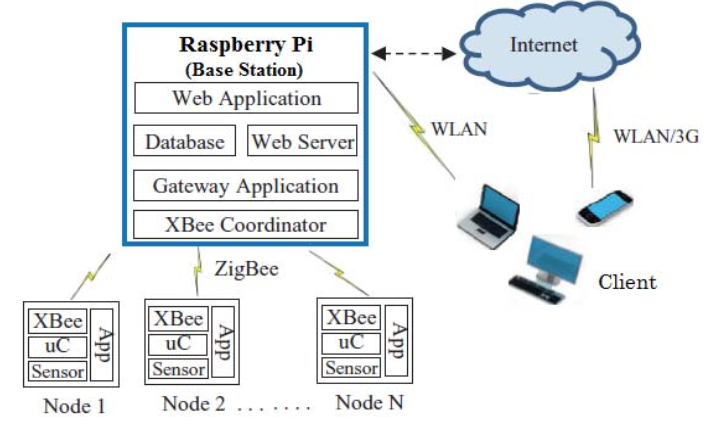
\includegraphics[width=\textwidth]{PiSystems.png}
    \caption{Rasberry PI based system 
    (\href{https://www.semanticscholar.org/paper/A-low-cost-environment-monitoring-system-using-Pi-Deshmukh-Shinde/e05a1fb72b08803d40dc06fa202241636fb82c21}{Image Source} \textcopyright ) }
    \label{fig:PI}
\end{figure}
\\

\indent \indent
By the time writing, TSC is an active research topic that proved to be really
challenging. Continuous work has been done on designing and developing
intelligent traffic signal control systems that could address the issue.\\
\indent \indent
So new methods and advanced systems and many other algorithms have
been proposed by the researchers to solve this TSC problem, mostly 
beeing based on fuzzy logic, evolutionary algorithms,
image processing, neural network, etc. \cite{Tomar2022}.
All of the methods aimed to reduce the overall waiting time and prevent traffic
jams from occurring while maintaining drivers safety. In this section we will
discuss about some of the methods that were put in to use and their ups and
downs. After describing each and every tehnology we will have a brief
comparison to highlight some of their characteristics.

% sectiunile devin capitole


\section{Object recognition based systems}
\indent \indent
One way to determine traffic scenarios was done with
the help of cameras. To be more specific we wanted to 
calculate the traffic waiting queue by detecting cars 
present int the images provided by our hardware components (Figure ~\ref{fig:ObjectRecognitionSystem}).
This problem was addressed by the help of vehicle tracking
and image segmentation algorithms.
\begin{figure}[h!]
    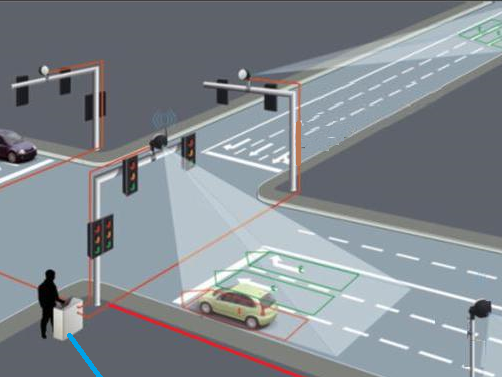
\includegraphics[width=\textwidth]{ObjectRecognitionSystemRepresentation.png}
    \caption{Object Recognition Based Traffic System Model 
    (\href{https://english.mathrubhumi.com/news/kerala/knowing-traffic-camera-locations-isn-t-enough-to-escape-from-them-mvd-can-move-them-easily-1.7427787}{Image Source} \textcopyright)}
    \label{fig:ObjectRecognitionSystem}
\end{figure}
\\
\indent \indent
However, the techniques used to solve the problem proved to 
be ineffective in real-time scenarios due to it's high
computational complexity that made the system unable to keep up 
with the traffic flow especially at high speeds.
Also, some are not even able to operate in bad weather conditions,
so they were doomed to failure. Studies had shown that whenever
visibility is reduced due to rain, fog or other external factors that
the pecentage of vehicles that will be detected will significantly drop.
\cite{Sheeny2021} \\
\indent \indent
Even if the problems stated above were known,
neural networks systems have been developed with the help of
object recognition algorithms.
They were designed to predict the upcoming traffic volume
from a X-min daylight traffic flow on different traffic conditions. 
Like so we would be able to overcome the high computational
complexity of the algorithm by avoiding 
recalculations. This lead to high memory needs,
that could not be overcomed, so this approach is
unsuitable for real-time systems. Also, we believe that it 
is almost unpossible to predict traffic on a constant manner, 
and our best way to handle it is to dynamically adapt to it.
We can still make use of a model that pools all traffic states 
for detection, but the actual "prediction" of the next traffic 
state should be calculated dinamically from real-time data.\\

\section{Vehicle sensor detection based systems}
\indent \indent
Another approach would be to collect data about the vehicles 
approaching junctions with the help of GPS sensors.
(Figure ~\ref{fig:SensorRecognitionSystem})\\

\begin{figure}[h!]
    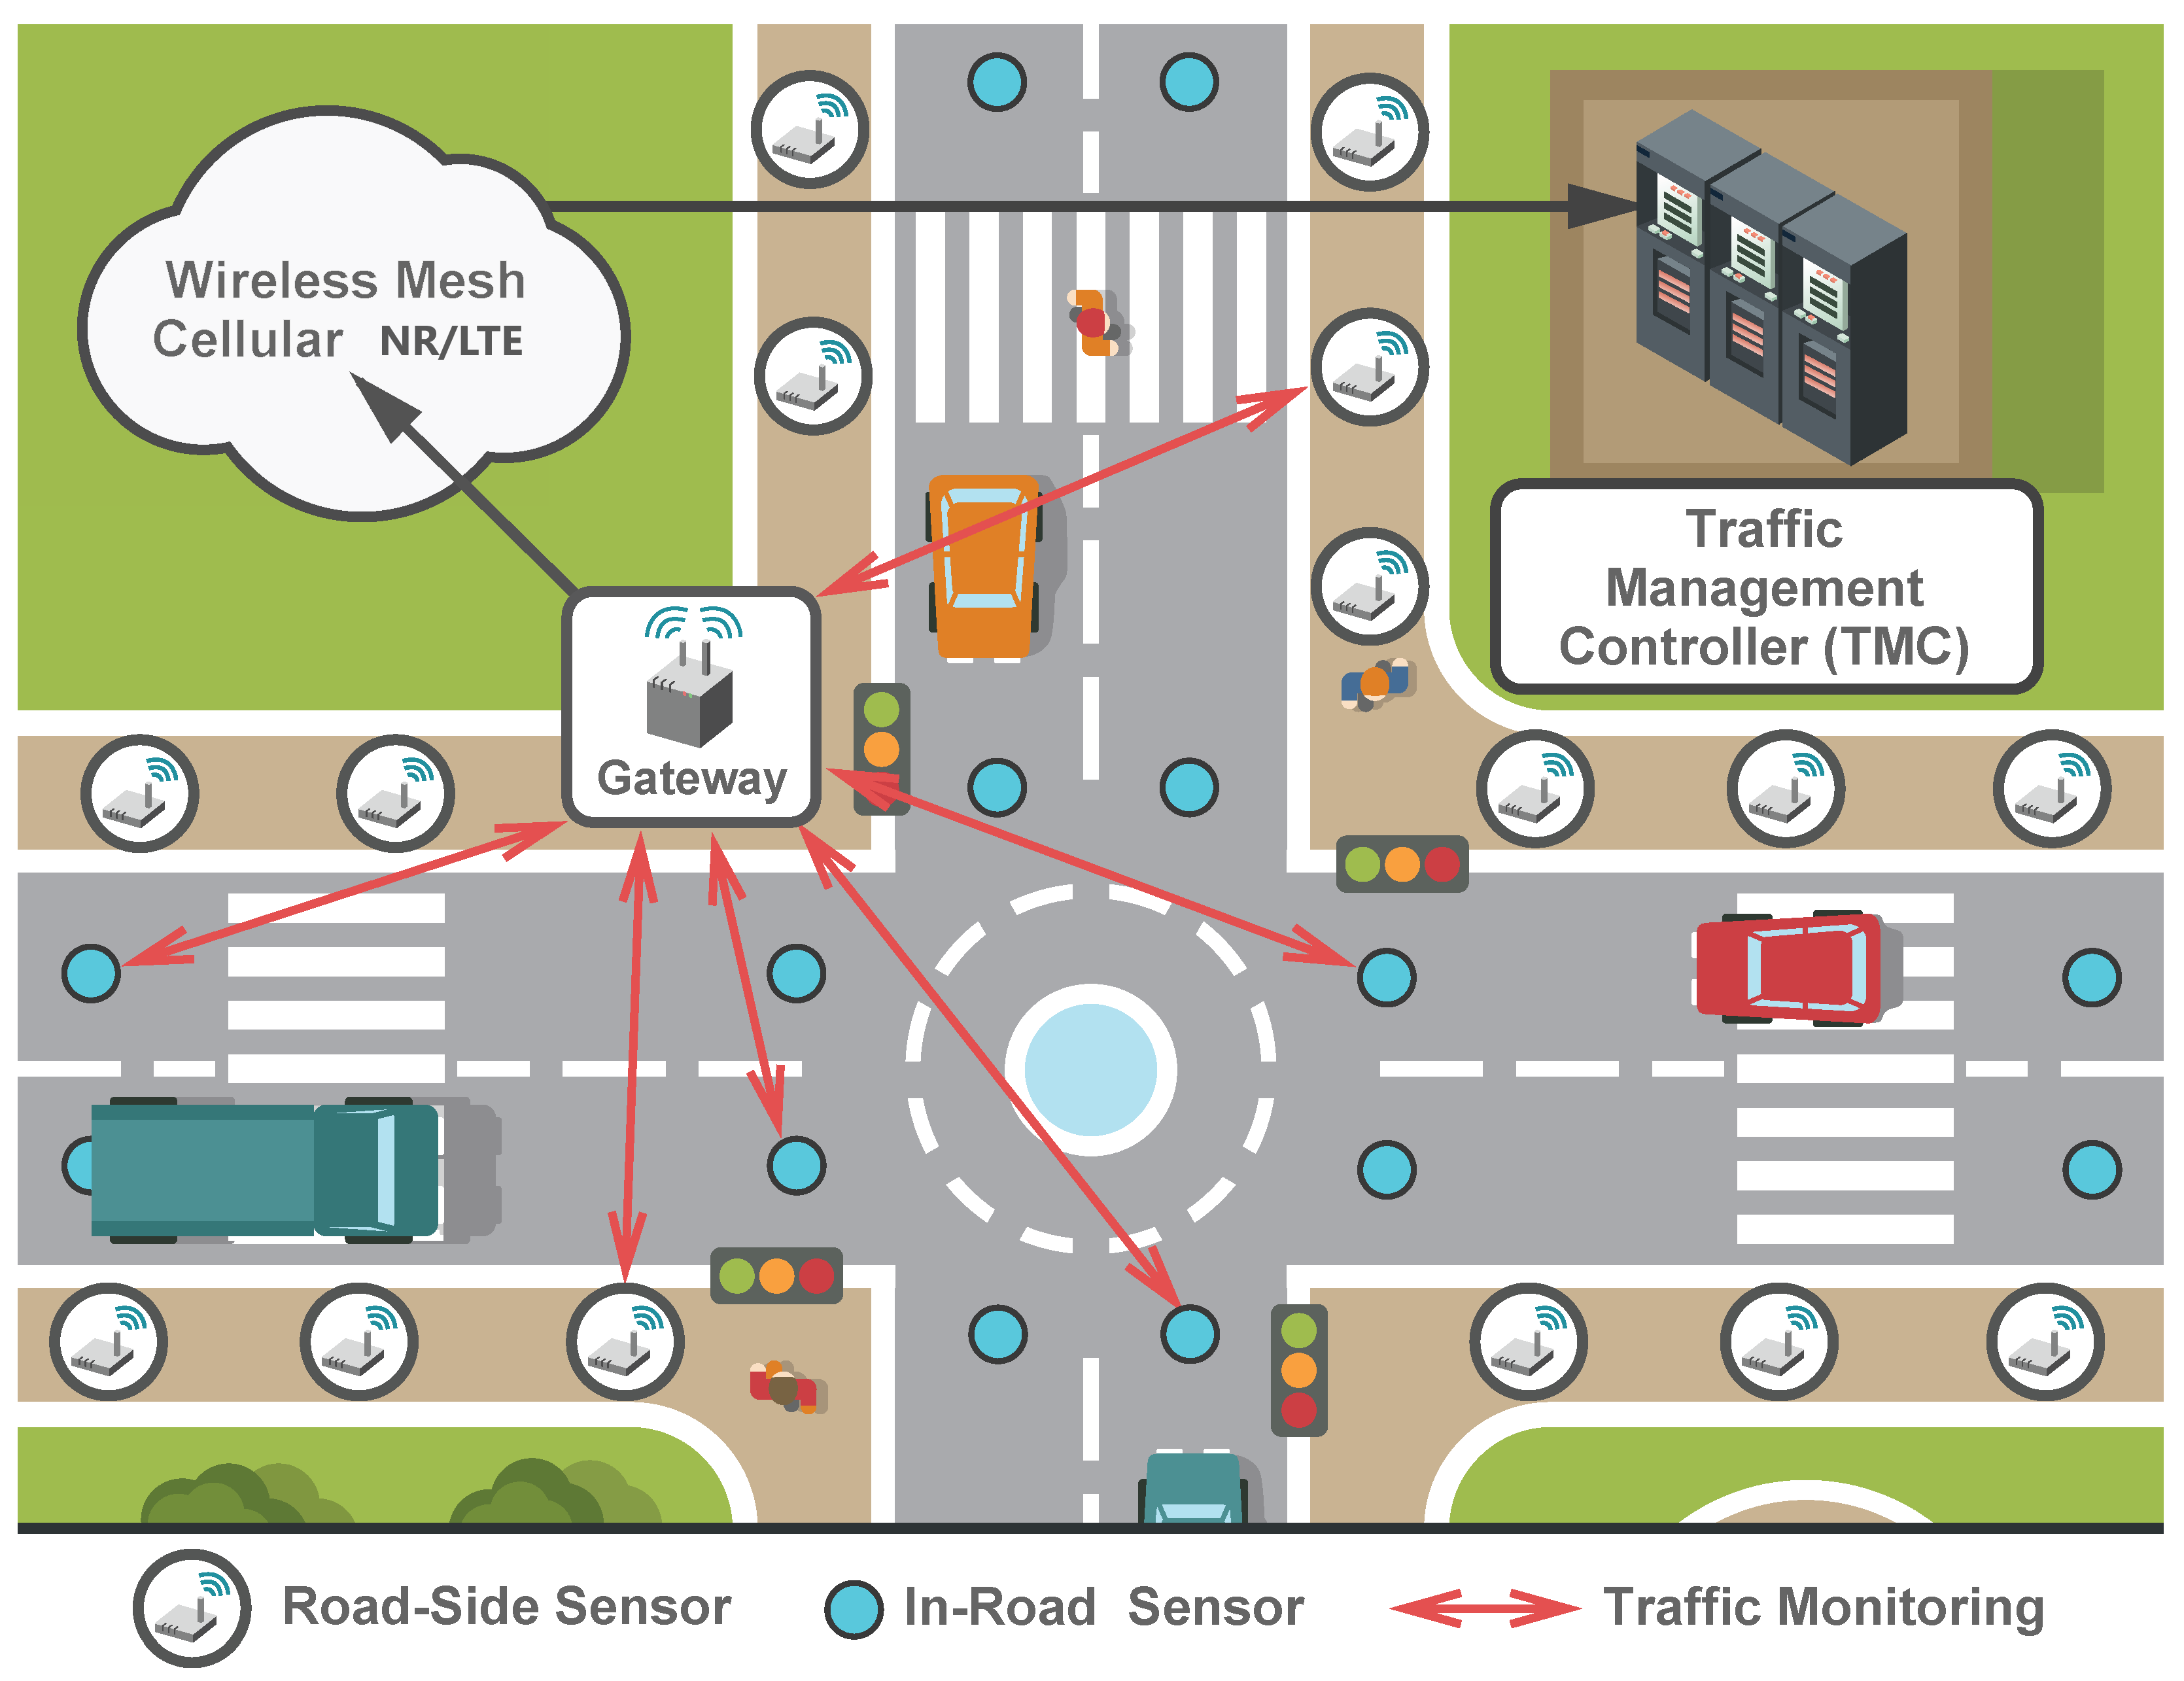
\includegraphics[width=\textwidth]{SensorsBasedTrafficControlSystemRepresentation.png}
    \caption{Sensor Based Traffic System Model 
    (\href{https://www.researchgate.net/figure/Communications-chain-of-data-feeds-in-smart-transportation_fig3_309740417}{Image Source} \textcopyright)}
    \label{fig:SensorRecognitionSystem}
\end{figure}

\indent \indent
One way to do it is to track the position, speed and direction of the given
vehicles. Sadly, this method would work only for a road network,
it can not solely control the traffic signal timing for just one junction. 
This is due to the high speeds that vehicles travel at and the time 
complexity of the  main algorithm.\\ 
\indent \indent
Another way to do it is to monitor the arrival and departure of vehicles at a
junction. This can be done with the help of sensors and traffic servers.
Like so we could use embedded technology to record the GPS data and send it to
the traffic monitoring system through GSM/GPRS. The drawbacks of this method
are the fact thats it involves very high implementation cost and, sadly, some
vehicles can not be tracked using radio detection systems. This problem can
be also aproached with the help of in-road sensors, but it would require even higher 
costs as you would need to often change the sensors because roads need to be
rebuilt due to wear or ongoing costructions periodically.


\section{Traffic Lights Synchronization based systems}
\indent \indent
Traffic Lights Synchronization (TSC) \cite{Tomar2022} systems aim  to minimize
the number of STOP and GO occurrences by adapting the traffic light phases at junctions.
This technique involves all vehicle maintaining a consistent speed while traveling on one side
of the road, allowing them to continue indefinitely to the opposite end of the road by consistently
encountering green lights at intersections by maximizing their number.
Studies had shown that in comparison with other fixed time and
non-synchronized traffic control strategies it reduces overall travel time by
up to 39\%. \cite{ALEKO2019}\\
\indent \indent
Just like most of the others methods, it collects and procces data from real traffic
scenarios to determine the green light timer. When vehicles pass through a juction the
green light timer for the following juctions decreases by a certain amount
(Figure ~\ref{fig:TrafficSignalSynchronization}). As with the other roads present at
the juction, the red light time increase to guarante the continuous motion of already
travelling cars. This can be done for mutiple levels of traffic depending on how many
junctions do you want to synchronize with one another, but must of the the times it
was handled as a 2 level system.
\begin{figure}[h!]
    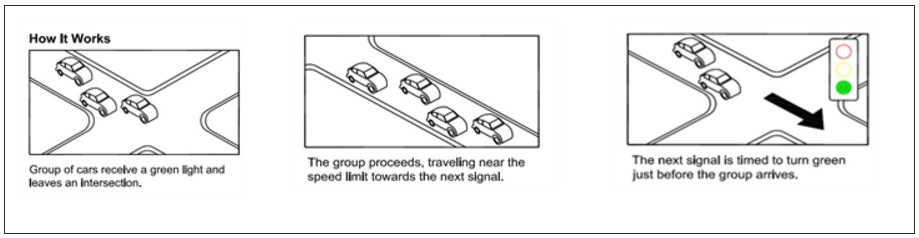
\includegraphics[width=\textwidth]{TrafficSignalSynchronization.jpg}
    \caption{Traffic Signal Synchronization Model 
    (\href{https://www.cityofirvine.org/signal-operations-maintenance/traffic-signal-synchronization}{Image Source} \textcopyright)}
    \label{fig:TrafficSignalSynchronization}
\end{figure}\\
\indent \indent
Multiple approaches to implement this kind of systems were made with the use of
varios AI algorithms and already known data collecting methods but the result are
mostly the same. This method would lead to longer red signal time, but will reduce
the overall waiting time when travelling long distances. One other advance to keep in
mind is that, as result of this phenomenon, the wear of the vehicles will be
drastically reduced.\\
\indent \indent
The main disadvantages of this method is the fact that you will eventually have to
prioritize one route. This would be problematic if multiple main roads collide with
one another. Also, the algorithm will not always provide an optimal solution as
drivers following sideroads may have longer waiting times. One more thing to keep in mind
is that this method is reliant on drivers speed consistency. Most of the cases, there 
will be a decent amount of speeding vehicles that will not be able to pass multile
junctions without any kind of stops as the algorithm itself does not intend to handle those 
edge scenarios.

\section{Fuzzy Intelligent Traffic Signal Control System}
\indent \indent
Fuzzy Intelligent Traffic Signal Control (FITS) \cite{Teo2010} \cite{Jin2017}
systems were originally designed to mimic a human policeman in controlling
traffic lights at an intersection. They are systems that take
different types of traffic input and apply fuzzy rules to 
manage the traffic. Like so data is converted into fuzzy truth
values between 0 and 1. For instance, the green light extension
time can be modeled by a number of fuzzy sets including “none”(1),
“short”(2), “moderate”(3) and “long”(4). The only thing that you are left to do is
to define your membership functions for the given set. For example we can
use the following functions to do so:\\

\begin{equation}
    "none" - f(q) = max(min((10 - q) / 10, 2), 0)
\end{equation}

\begin{equation}
    "short" - f(q) = max(min(q / 10, (20 - q) / 10), 0)
\end{equation}

\begin{equation}
    "medium" - f(q) = max(min(q / 5, (30 - q) / 5), 0)
\end{equation}

\begin{equation}
    "long" - f(q) = max(min((50 - q) / 10, q / 2), 0)
\end{equation}


Like so we would alternate base on other fuzzy values or randomly, between
choosing "none", "short", "moderate" and "long" fuzzy values, to determine 
the time that our green light should last.\\
\indent \indent
Depending on the actual improvements of the traffic flow the algorithm will 
adapt, altering it's member functions and decreasing/increasing the odds to 
chose one specific fuzzy value from the set. One big advantage that this would 
lead to is that FITS mitigates the negative effects of detection malfunction
by predicting the traffic states at the whole intersection by simulating real
time traffic scenarios. So FITS may be able to run withot any kind of additional
hardware, leading to huge cost advantages.\\
\indent \indent
Despite all of the bennefits presented above, as with any AI based algorithm,
it takes a lot of time for the algorithm to improve itself and the upgrade.
Also the chance to upgrade is very reliant on traffic conditions. Furthermore, 
even if the algorithm has been running for a long time, it still can choose a
non optimal solution that may or may not lead to traffic jams. 

\section{Dedicated Short-Range Communications systems}
\indent \indent
To explain why this kind of systems would work, first we have to understand what
are Dedicated Short-Range Communications (DSRC) \cite{Zhang2018}
\cite{Tomar2022}. DSRC are one-way or two-way wireless communication channels
specially designed for use in automobiles that are mostly used by ITS to
comunicate with other vehicles or infrastructure technology. They operate on
the 5.9 GHz band of the radio frequency spectrum and are effective over short
to medium distances.\\
\indent \indent
One technique that was developed with the help of DSRC is the Virtual Traffic
Light (VTL) approach. VTL is a biologically-inspired approach to traffic
control that relies on Vehicle-to-Vehicle (V2V) communication by using the
Signal Phase and Timing (SPaT) message and Basic Safety Message (BSM) from
the DSRC OBU. (Figure ~\ref{fig:DSRCRadio})
\begin{figure}[h!]
    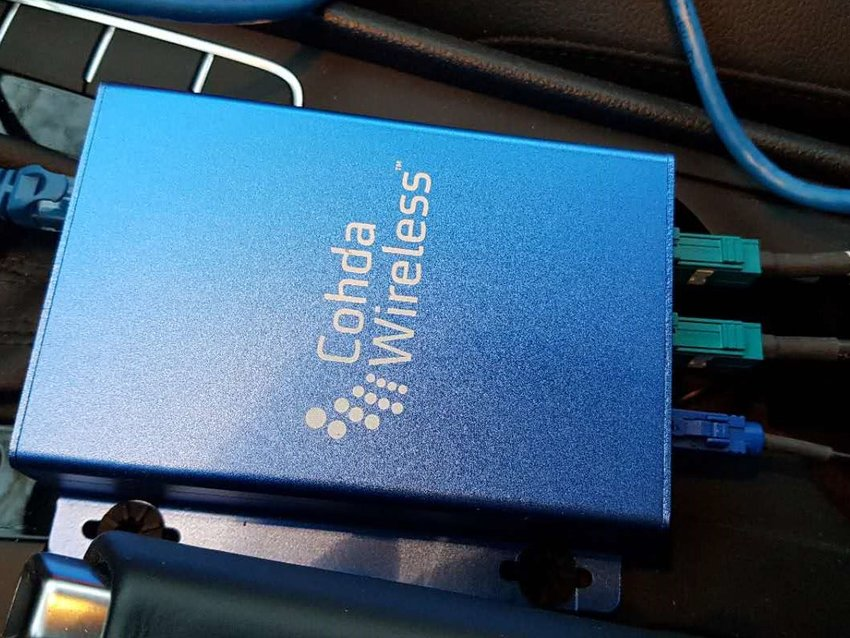
\includegraphics[width=\textwidth]{DSRCRadio.png}
    \caption{Dedicated Short-Range Communications Radio 
    (\href{https://www.researchgate.net/figure/DSRC-radios-used-in-the-prototype-system_fig1_326198424}{Image Source} \textcopyright)}
    \label{fig:DSRCRadio}
\end{figure}\\

\indent \indent 
The radio is capable of broadcasting several messages defined by the SAE 2735
\cite{Kenney2011IOT} protocol with the most important beeing BSMs. This kind of 
messages contain vehicle's current information (GPS location, speed and heading) that are associated with a temporary ID. As a result, by broadcasting
BSM messages we are able to detect the vehicles approaching the intersection in a
continuous manner, unlike traditional methods that only detect the presence of the
vechile using loop detectors.\\
\indent \indent 
You can image the cars beeing "moving routers", and the junctions beeing
"stationary routers". Whenever one "gateway" or in our case one traffic route is
overfilled with vehicles it blocks the others and starts letting them pass just like
RIP protocol. Like so we are not actually introducing new sorts of technologys that may
or may not fail, we just adapt already existing algorithms, that proved to be great
solutions, to fit one specific use case.

\begin{figure}[h!]
    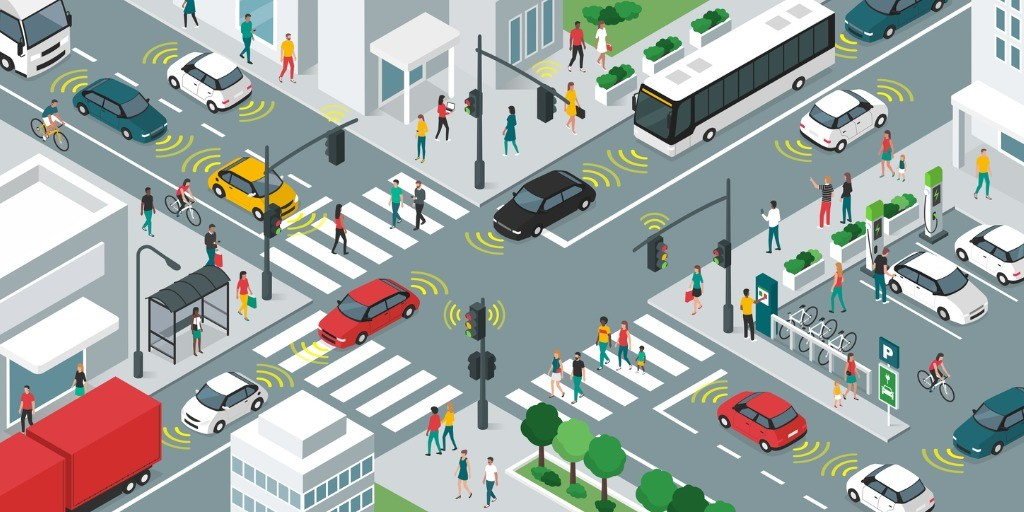
\includegraphics[width=\textwidth]{DSRCSystemModel.jpg}
    \caption{DSRC Based System Model 
    (\href{https://www.frost.com/frost-perspectives/what-is-required-for-a-scalable-and-industry-wide-vehicle-to-everything-v2x-deployment/}{Image Source} \textcopyright)}
    \label{fig:DSRCSystemModel}
\end{figure}

\indent \indent
With the help of this approach we can drastically reduce
the implementation costs as it does not require any kind of additional
expensive hardware components. Furthermore, it is robust against weather conditions
and easy to mantain. Extensive simulations have shown that this kind
of technology can reduce daily commute time in urban areas by more than 30\%.
Different aspects of VTL technology, including system simulation, carbon
emission, algorithm design and deployment policy have been researched in the
last few years. \cite{Neudecker2012}\\
\indent \indent
The main drawback of this approach is that it requires vehicles
to support DSRC technologies, which might me problematic at the given time.
Moreover, within V2V communications in VTL systems, there is a possibility of
encountering partial obstruction by physical object present in the innermost
Fresnel zone (non-LoS conditions). This presents a significant challenge in terms
of making quick decisions effectively. However, even if DSRC
technology isn't totally supported by vehicles and we might colide with non-Los
conditions, it proved to be effective in reducing the average waiting time at
juctions. So, maybe the next step on improving traffic flow, would be to create
an infrastructure for this kind of technologie, but only time will tell. In the mean
time the best thing we can do is to develop an economically efficient plan for
transitioning from existing traffic control systems to  VTL systems.

% de pus aici chapter cu motivatie
\pagebreak


\chapter{A new flexible economic approach}
\indent \indent
We belive that the future of traffic light management will be
based on DSRC like signals. No matter if it will still be based 
on DSRC, 5G or even 6G will take lead, we aim to provide a some kind of
software system that would be able to handle any kind message based 
tehnology. Also, because at the given moment, the infrastructure for
DSRC systems hasn't been fully developed and deployed we want to
provide a economic approach to the given problem that would bennefit
on the already working systems, but also can simulate the already
working traffic light management protocol.\\
\indent \indent
Even if DSRC will be fully deployed on a globas bases, there will still be
alot of poor countries that will have a hard time upgrading their infrastructure.
Because of that, we wanted to be able to have a working system even without 
investing any kind of money. Think about a PC for example, even one of the worst
ones can run an OS and if you want to updgrade them, to make it run faster or
handle a newer software, you would just add or replace a component with a better
performing one. Not only you will be able to add "performance boosts" as needed
to your given infrastructure but think about the scenarios when something goes bad?
What if one of your component goes down and for example the traffic light will
be stuck on red until someone comes and fixes it. That would lead to a
HUGE traffic jam.\\
\indent \indent
We also want to be able to take advantage of already working DSRC compatible
vechiles without adding any kind of new hardware  and be able to 
disable the additional protocols and move to a fully DRSC based
system if needed.

Sounds great, right? This is how we designed it. The system will have \textbf{4 major
components}: \textbf{2 types of clients}: one stationary one and one moving one, 
"attached" to our vechiles; \textbf{2 types of servers}: one that would manage the
position of the clients and redirect them to the corresponding servers
and one that would handle all of the messages and change the actual traffic lights.
For the simplicity on things we will name them as follows:
\begin{itemize}
    \item \textbf{Traffic Observer (TO)} - the stationary client.
    \item \textbf{Vehicle Tracker (VT)} - the moving client installed on our vehicles
    \item \textbf{Junction Main Server (JMS)} - the server that handles the traffic lights
    \item \textbf{Proxy} - the server that will guide the clients to the corresponding
    servers
\end{itemize}

The system would work as follows: We would constanly have a TCP-IP connection
between our clients and the corresponding JMS. Once they are connected
clients would send various data about the traffic that would be further 
proccesed by the JMS and traffic lights would be changed accordingly. The
TO would be responsible for sending data about the traffic on it's road and the 
VT would be responsible for sending it's own data to the server (Figure ~\ref{fig:UC_DiagramAll}). 
We also handled the cases when there is an emergency ongoing like any kind of
special vehicles crossing the junction but we will talk later about this
because it requires some more attention as it can be easily exploited if not 
handled right. Just imagine any kind of cars beeing treated like an ambulance
on duty, you would just be able to pass freely any kind of junction without 
ever waiting at the red light.\\

\begin{figure}[h!]
    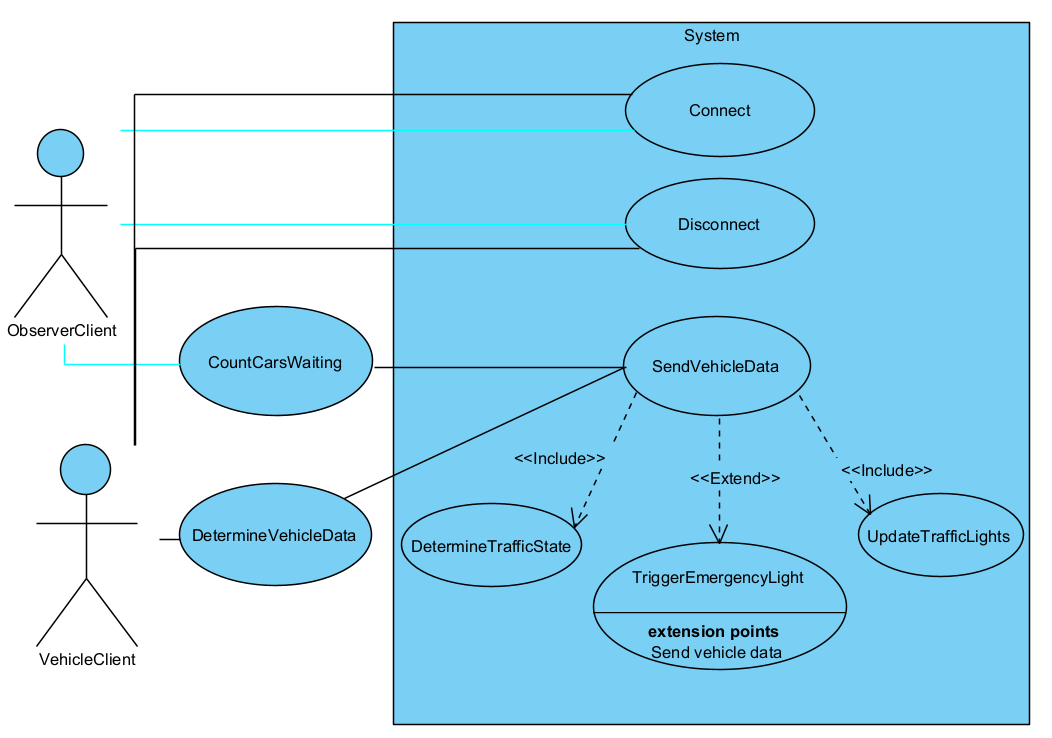
\includegraphics[width=\textwidth]{UC/UCDiagram.png}
    \caption{All UC Diagram}
    \label{fig:UC_DiagramAll}
\end{figure}

\pagebreak

\section{Proxy}
\indent \indent
The first problem that needs to be addressed is the fact that VTs will 
constanly have to switch between JMSs, but how do we know what server to 
connect to? We do not want to connect to each and every server in the 
covered area and start broadcasting mostly useless message. The answear
would be that each client will know the main server off the system, that
would act just like a proxy and redirect them to the corresponding JMS.
For that we would need to store the JMS coordinates in one or multile
database. The VT would need to just send its own coordinates and the
direction they are heading, as a result the proxy would provide de IP
address of the corresponding JMS (Figure ~\ref{fig:UC_Connect}).\\
\indent \indent
As we want this to be scaled on a global level, the system supports
horizontal scalling, as we can just stack proxys one on top of the 
other and instead of having stored only the JMS coordinates we 
will also store all the proxys that are in the subarea of the owner. To 
not overload any kind of servers we also implemented a load balancing
mechanism that prevents this kind of issue.
\begin{figure}[h!]
    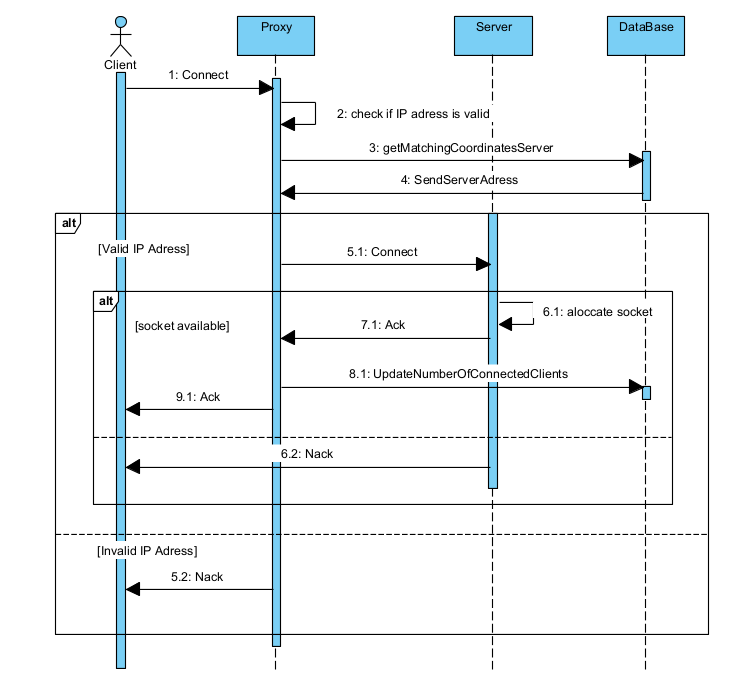
\includegraphics[width=\textwidth]{UC/Connect.png}
    \caption{UC: Connect}
    \label{fig:UC_Connect}
\end{figure}

\pagebreak

One thing this can lead to is a 
better surveillance of the vechiles that aren't suppose to be on the 
road in the first place. The IP address of a given vechile can be "banned"
and if it tries to connect to the JMS the message will be ignored
and not only the JMS will not count the waiting vechile, sometimes 
leading to longer waiting times for the individual that is driving the
vechile and broke the law, but also like this we would have the proof
that he broke the law so we would be able to further punish him. We can lower the number of cars driving on the public
roads that do not respect safety norms and reduce the number of
accidents. For this to work we will need to also disallow owners to 
change their hardware without any kind of approval as a new radio
would lead to a different serial number and this would be problematic.\\
\indent \indent 
Once passing the area of coverage of that given junction we would also need
to disconnect from that given JMS (Figure ~\ref{fig:UC_Disconnect}). By doing 
this we will be able to always track the vehicles and react accordingly when
one or multile leave the junction. One thing that we have to mention is that if
we further think about this we could in theory keep a constant track of ALL
the vehicles ON A GLOBAL BASES and no longer require licence plates, if, of 
course all the vehicles would support sending DSRC signals.  

\begin{figure}[h!]
    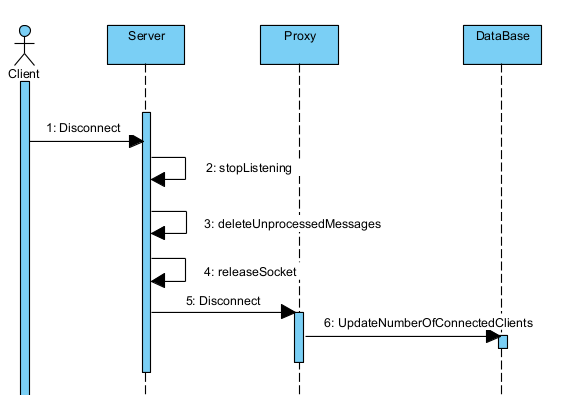
\includegraphics[width=\textwidth]{UC/Disconnect.png}
    \caption{UC: Disconnect}
    \label{fig:UC_Disconnect}
\end{figure}

\pagebreak

\section{Traffic Observer}
\indent \indent
The second thing we need to do is provide a way to detect the
waiting vechiles withot the help of DSRC messages. This can be
done in mutiple ways, but for the simplicity of things and to keep
costs as low as possible we went with an camera based system.
The way it works is as follows: multiple cameras are mounted on the road 
that are connected to microcontrollers, we take the images provided and 
apply object recognition algorithms to detect the passing cars.

\begin{figure}[h!]
    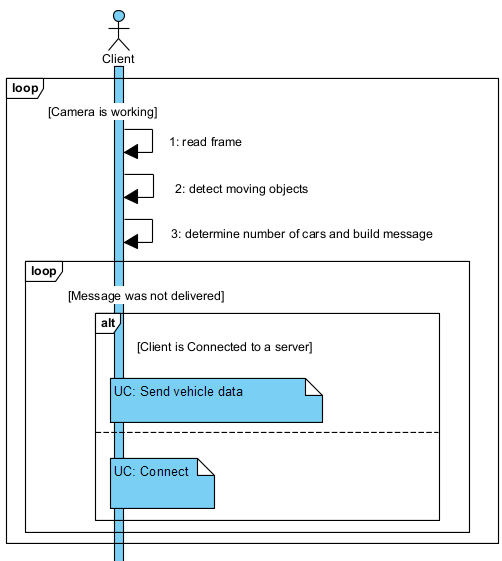
\includegraphics[width=\textwidth]{UC/ProcessImageAndFindTheCars.png}
    \caption{UC: Find cars from provided images}
    \label{fig:UC_FindCars}
\end{figure}

\pagebreak
The first thing we actually do is preprocess the given images and 
detect the moving objects inside our frames and second of all
determine if that moving object is or is not a vechile (Figure ~\ref{fig:UC_FindCars}).
Like this we can speed up the image detection process as we will have less pixels
to keep track off. This overall speeds up the system as can be seen in
Figure ~\ref{fig:Comparison}. The blue line represents the amount of cars 
detected with it running and the red one without it.
%TO PROVIDE REAL DATA WHEN APP IS DONE
\begin{figure}[h!]
    \centering
    \begin{tikzpicture}
        \begin{axis}[
            xlabel={$seconds$},
            ylabel={$cars-counted$},
        ]
            \addplot[color=red]table {testData/dataNoMovementRecognition.txt};
            \addplot[color=blue]table {testData/dataMovementRecognition.txt};
        \end{axis}
    \end{tikzpicture}
    \label{fig:Comparison}
    \caption{Car tracking performance}
\end{figure}

\section{Vehicle Tracker}
\indent \indent
We want to be able to be able to send DSRC signals from any given vehicle.
To do that, we make use of already integrated hardware components, to be more
specific we make use of the radios and GPS installed on our vehicles. Like this,
we get the coordinates of the vehicle as well as it's heading and the radio
allows us to establish TCP-IP connection and send messages. So the only things
that is left to do is to download our service and keep it running while travelling.\\
\indent \indent
Whenever a vehicle wants to connect to a junction, it will have to specify it's 
serial number, like this we will be able to deny/accept it's connection. The only 
tricky part that is left to do is prevent anyone from changing thir serial number.
This can be done in many ways, like changing the ACL of the executable to be 
ran or overwritten only by the system or simply putting a flag in memory to 
prevent any kind of acces in the location where the executable itself is stored or 
just encrypt the whole storage space of the vehicle. The security part of the
system itself is not yet defined, it will be developed only if the project will gain momentum.
\pagebreak
\section{Junction Main Server}
\indent \indent
To handle all of those messages and change the actual flow of traffic we
need to have a main command unit that acts as a server. Now 
that we know about all the components of the system we can 
start vizualing it(Figure ~\ref{fig:System_sketch}). Clients will query the 
2 time of servers and connect their corresponding junction. Once connected, 
they will send varios type of data to the junction server and the server itselft 
will change the traffic phases based on the data recieved.

% de facut poza mai mica si bagat text eventual
\begin{figure}[h!]
    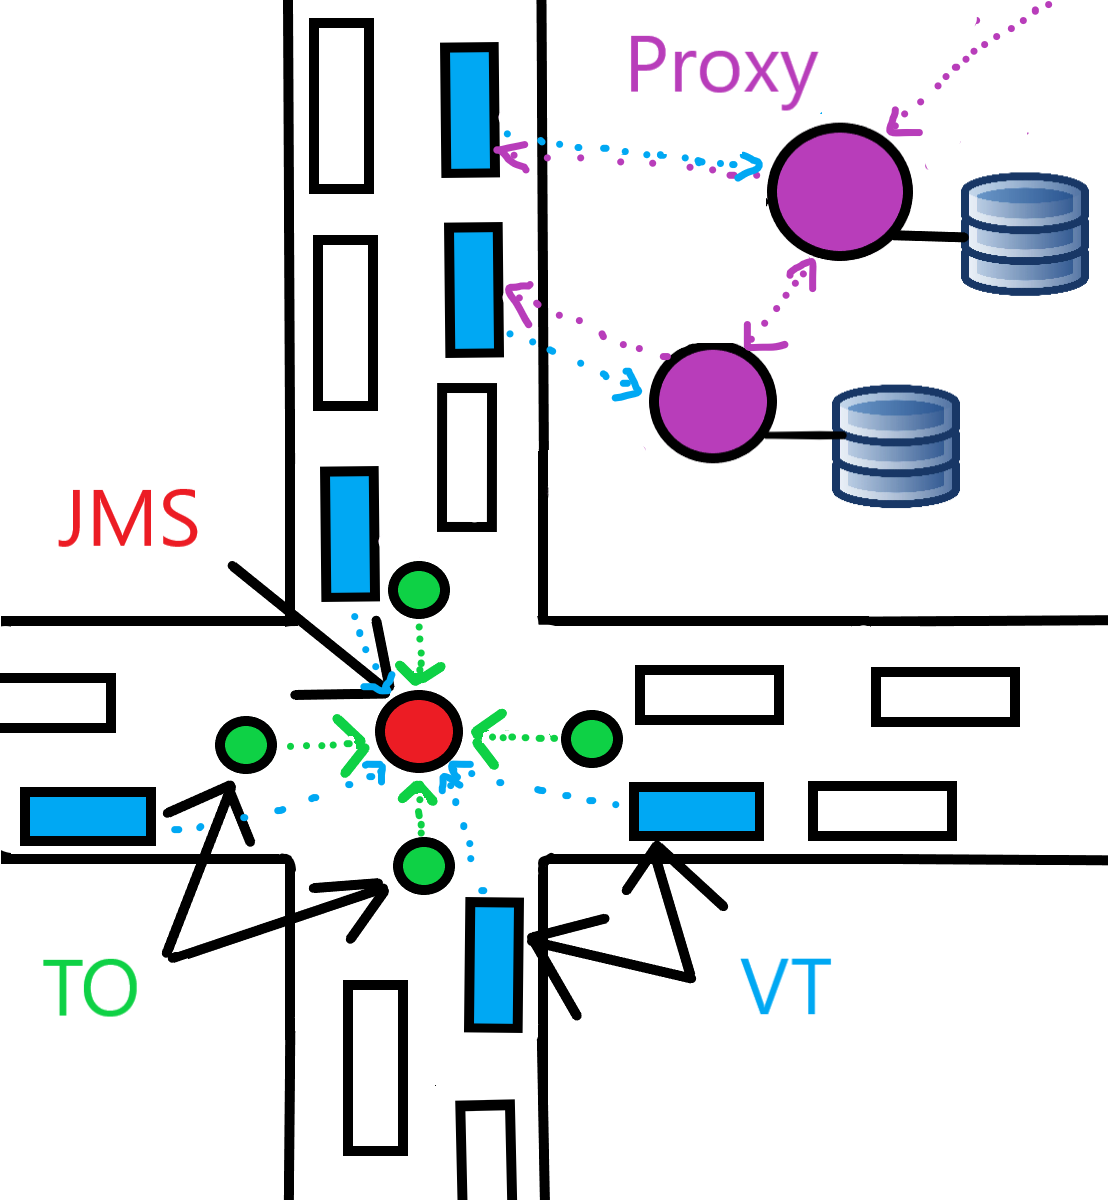
\includegraphics[width=\textwidth]{Sketches/SchitaSistem.png}
    \caption{System sketch}
    \label{fig:System_sketch}
\end{figure}

\pagebreak

\begin{figure}[h!]
    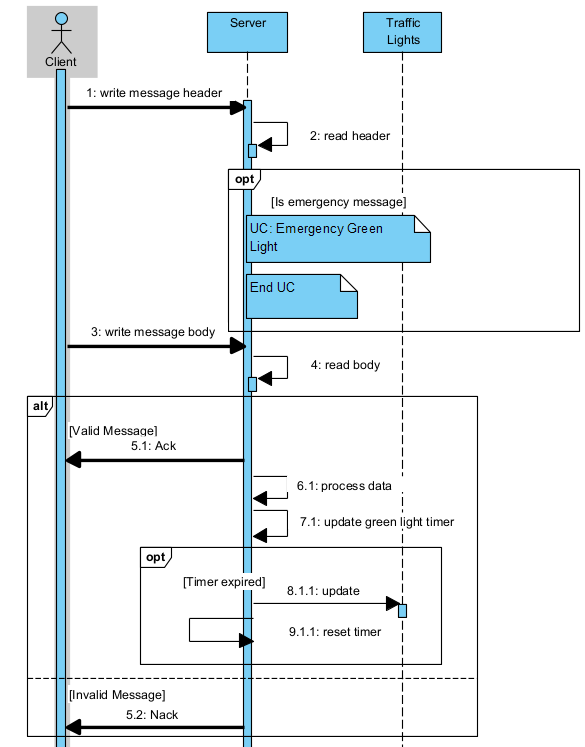
\includegraphics[width=\textwidth]{UC/SendVehicleData.png}
    \caption{UC: Send vehicle data}
    \label{fig:UC_SendVehicleData}
\end{figure}

The mechanism works mostly like any other TCP-IP mechanisms.
We read the header of the message to determine the type of 
message recieved and the size of the actual message then
based on the info we procces the data and update the traffic 
state. You may ask what happens if a car is detected by the 
TO as well as it's data is sent to the JMS trough a VT.
Well, because of this scenario we chose to aproximate the 
traffic based on the number of cars determined by the TO 
and the number of VT that sent messages to the JMS. Like this
we make sure that, if one of the 2 components or both fail the system
will still work. Also because noone is suppose to wait to long
for the green light we can set a maximum timer for the red light.
Imagine beeing alone on one road waiting for the green light and
having thousands of cars crossing the intersection from another road,
you would have to wait ages for you to be able to cross. This prevents that
and acts just like an "aging mechanism" (Figure ~\ref{fig:UC_SendVehicleData}).

\begin{figure}[h!]
    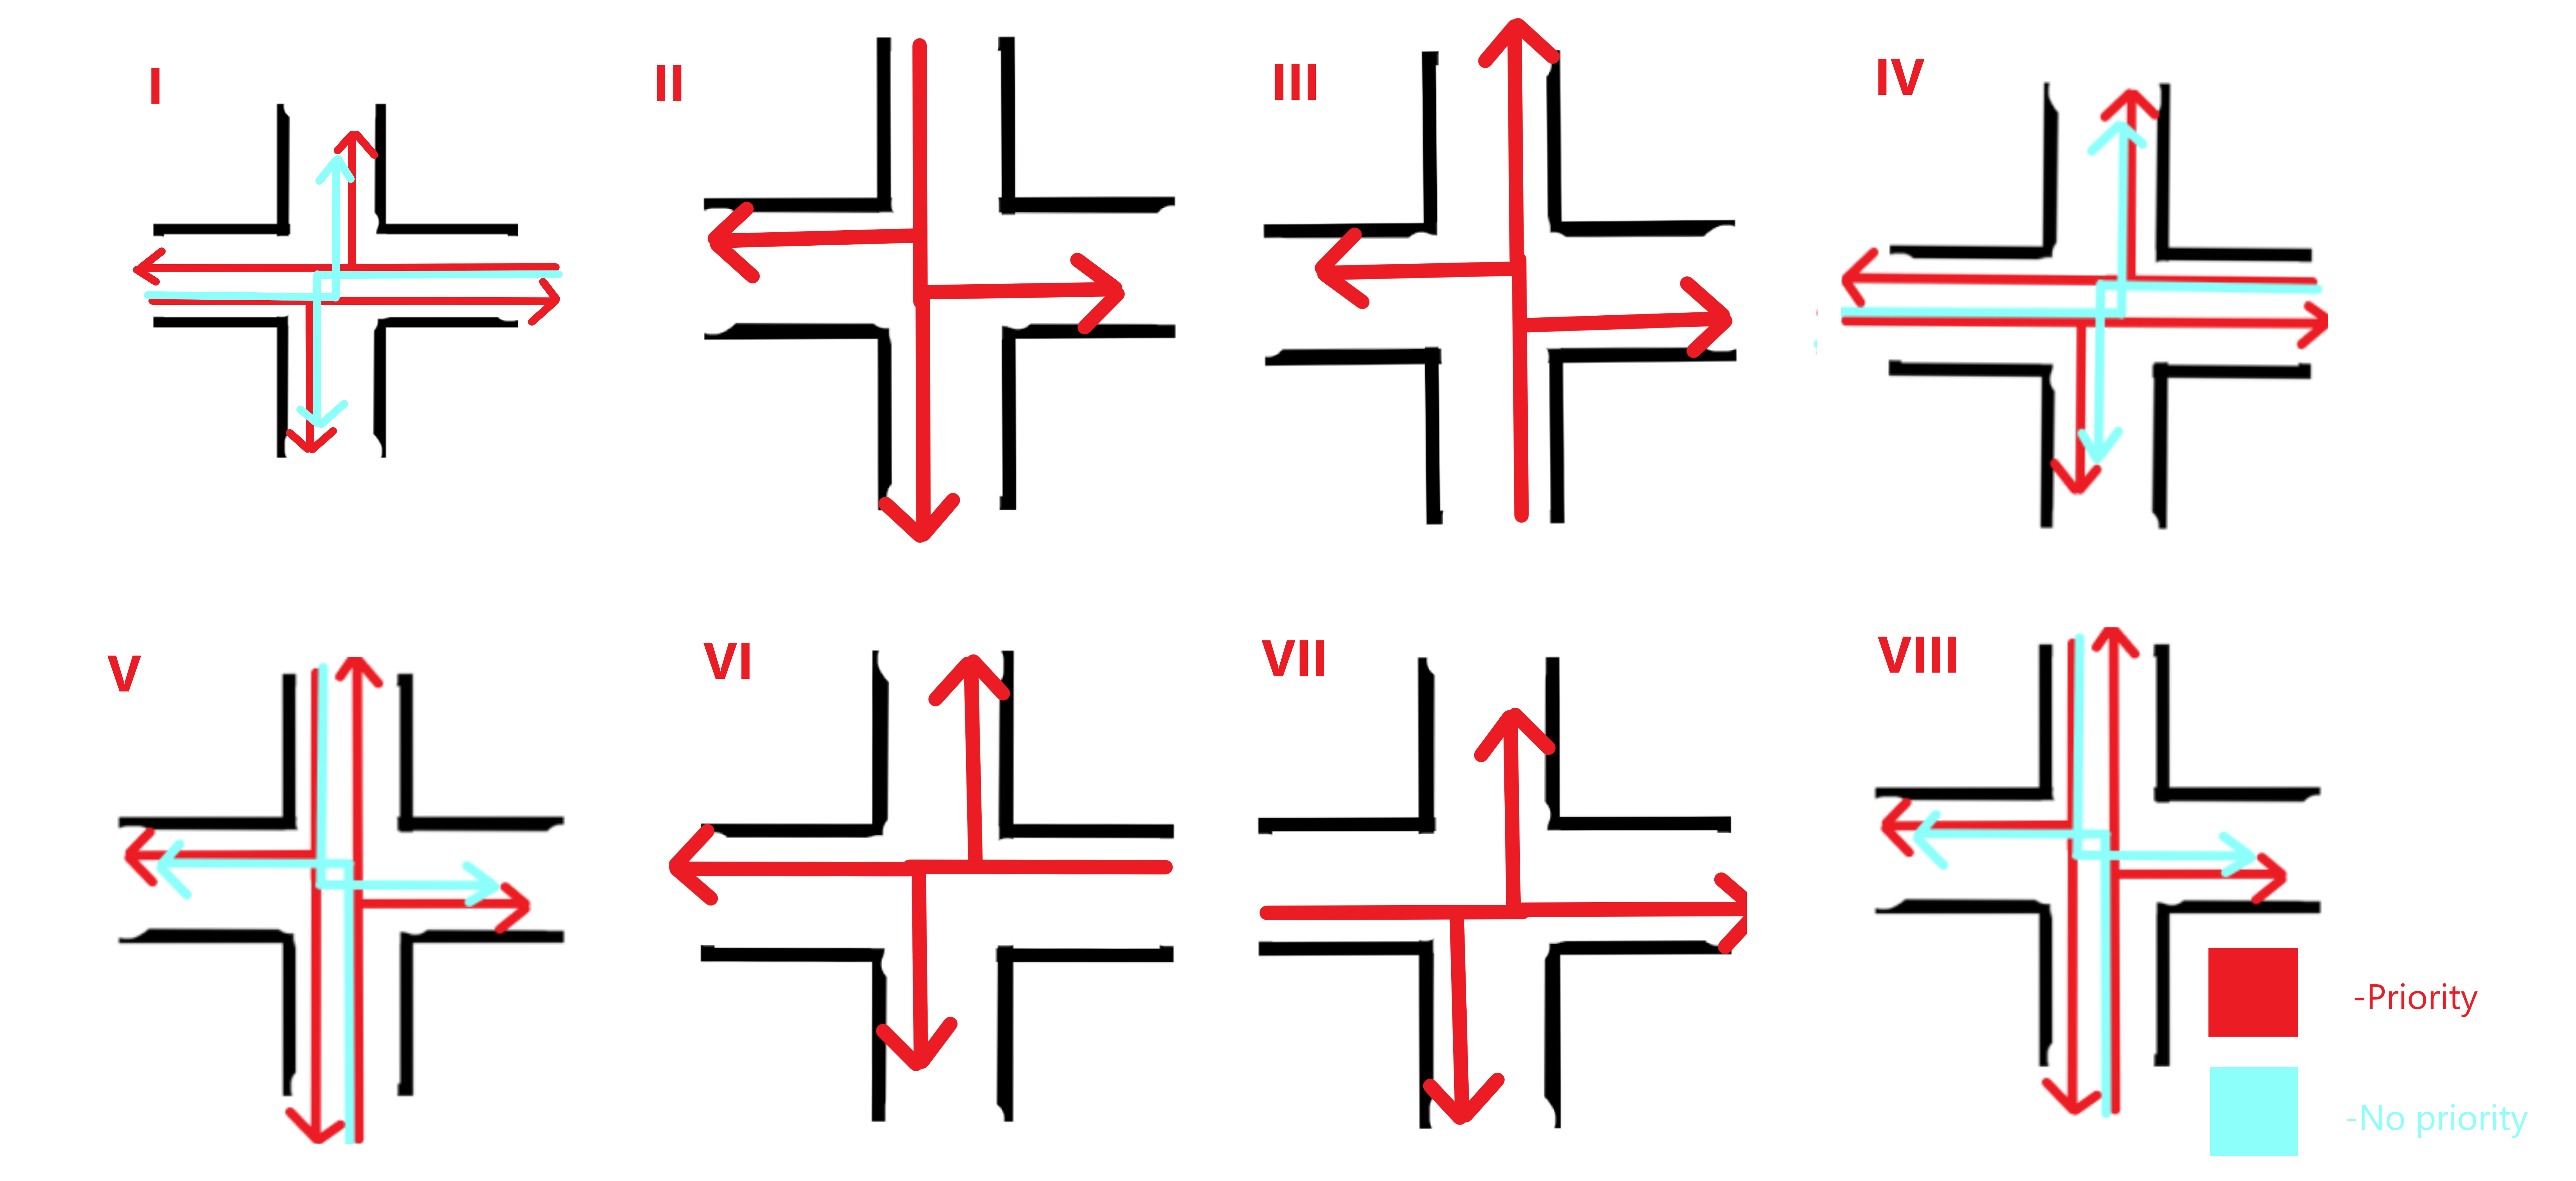
\includegraphics[width=\textwidth]{Sketches/AvailableJunctionPhazes.png}
    \caption{Junction Phazes}
    \label{fig:Junction_Phazes}
\end{figure}

As far as the main algorithm for the traffic management goes we have 8 phazes of
the traffic (Figure ~\ref{fig:Junction_Phazes}). The most basic scenarios is that the 
traffic will follow that 8 phaezes going trough phaezes 1 to phaze 8 in order and cycle. That's
the implementation for the way the traffic works, but we want to also be
able to jump from one phaze to any other at any given time, to be able to shorcut
the system. For that we are basing on several things.\\

\indent \indent
First and foremost we need to take into 
account the number of cars waiting. We do that by combining the provided data from the 
VT and TO and calculate an average of cars waiting.

\indent \indent
Second of all we will need to fully understand our traffic pahzes, why the are required
and how to determine the phaze we want to switch to. For that we first described the 
phazes based on the acting vehicles.\\
\begin{itemize}
    \item PHAZE I: E + W waiting vehicles
    \item PHAZE II: N waiting vehicles
    \item PHAZE III: S waiting vehicles
    \item PHAZE IV: E + W waiting vehicles (same with PHAZE I)
    \item PHAZE V: N + S waiting vehicles
    \item PHAZE VI: E waiting vehicles=
    \item PHAZE VII: W waiting vehicles
    \item PHAZE VIII: N + S waiting vehicles (sane with PHAZE V)
\end{itemize}

\indent \indent
We want to know when to switch from one phaze to another. For that we will have
timers for each direction: E, W, N and S. At first all the timers will be set to 
a costum amount, but the waiting time will be changed dinamically based on the 
traffic conditions as well as the green light waiting time.\\
\indent \indent
To start the whole mechanism we want to initiate the traffic as usual, 
having the normal order of phazez running and for us to switch to and abnormal 
phaze we'll just need one or more timers to expire. The check for the jump to an abnormal phaze
will be done ONLY when GREEN LIGHT ENDS.\\
\indent \indent
Last but not least we need to define the way our algorithm jumps from one phaze to 
another, for that we will use the following example
(Figure ~\ref{fig:PhazesSwitchingExample}):
\begin{figure}[h!]
    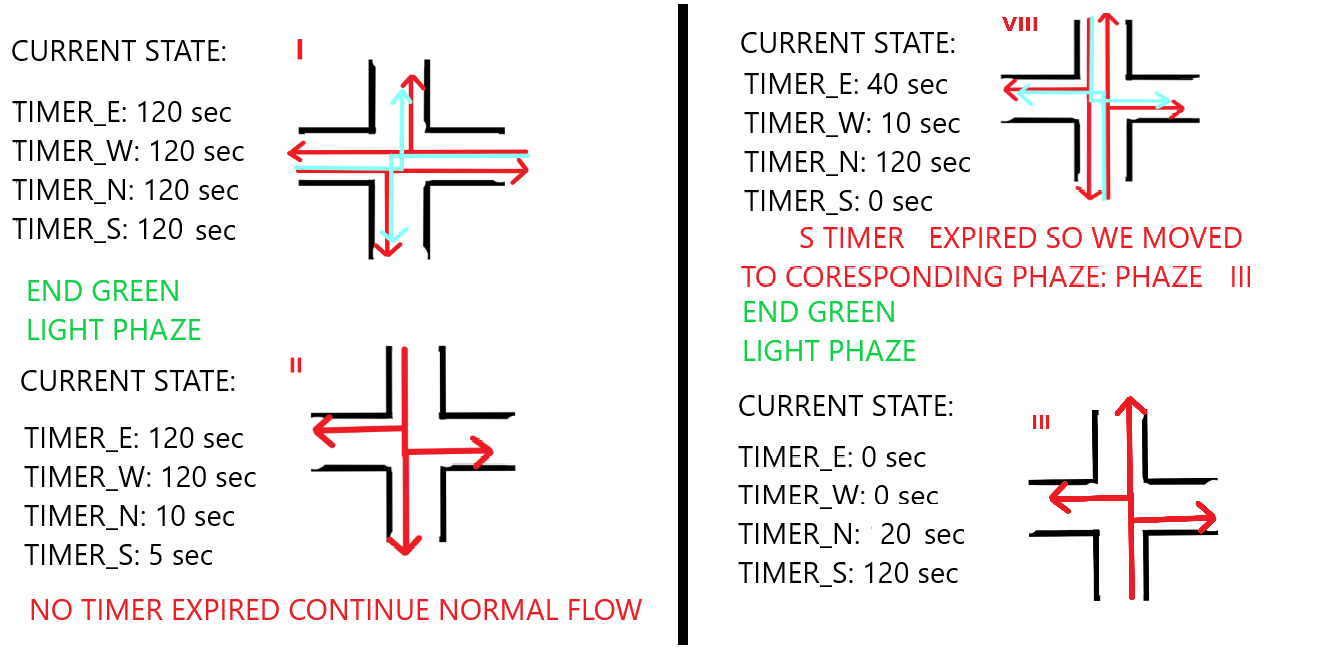
\includegraphics[width=\textwidth]{Sketches/SwitchingTroughPhazesExample.png}
    \caption{Phaze switching example}
    \label{fig:PhazesSwitchingExample}
\end{figure}
\\
\indent \indent
At the end of every green light phaze we check the timers. If any of 
them expired we jump to it's corresponding phaze. If, for example the following state
coresponds to the phaze we want to jump to, we do not short circuit the normal flow of
things. Every time we are trough green light phazes the timers corresponding to 
each lane that has a green signal is frozen and afterwards reseted.\\
\indent \indent
There are also "traffic conflicts" that can occur, for example, what if 
both the timers from E and S lanes has expired, we can not give a green light 
to both lanes, there isn't a corresponding traffic state. This are the edge 
scenarios that we want to avoid the most. The way we handle them at the given moment is 
that we just use FIFO logic, take the timers that expired first and build an existing traphic 
phase. When this happens we afterwards update the green and red light timers 
duration accordingly to prevent any more occurances. An example of the given 
scenario can be seen in Figure ~\ref{fig:FaultyPhazeSwitching}. 


\begin{figure}[h!]
    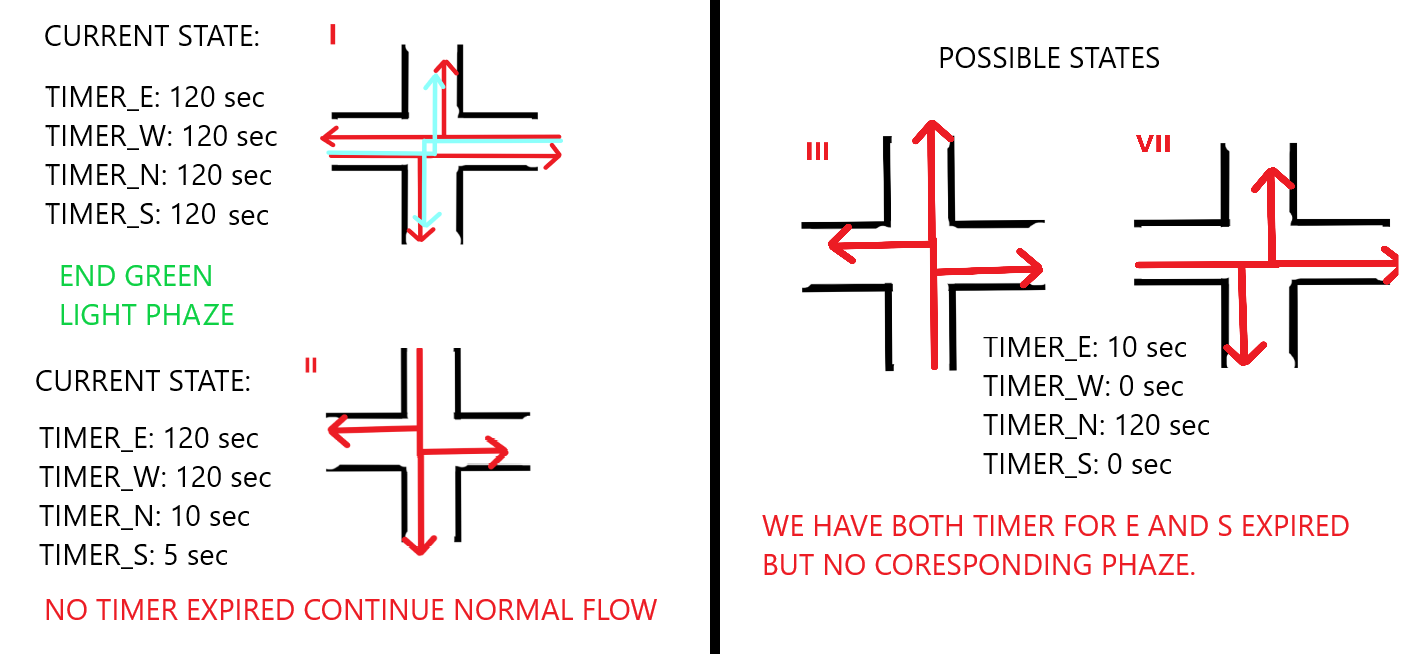
\includegraphics[width=\textwidth]{Sketches/PhazeSwitchingCaseToBeAvoided.png}
    \caption{Faulty phaze switching}
    \label{fig:FaultyPhazeSwitching}
\end{figure}

\section{Emergency states}
\indent \indent
The system also recognizes and treats accordingly
special vechiles like ambulances, police cars and fire trucks
crossing the junctions. Whenever one of those vehicle is detected
our server turns on the green light corresponding to the lane they are
following and keeps it on until it crosses the junction. This is called 
and emergency green light state. If we are already
in one to begin with, we will queue the next state by using FIFO rule.
The whole communication is done only by using VTs as the process of detecting 
special vehicles in mission would take to much time when it comes to object 
detection algorithms and time is key for us in those critical moments.
When no more emergency vehicles are present, tarffic will just go 
back to it's original flow, from where it left off.

\pagebreak



\chapter{Implementation details}
\indent \indent
The whole system was developed using C++17, Python, Boost, GLFW, MSVC WinAPI, OpenCV,
Tensorflow  and MySQL. The system itself is treated as a big project 
and splitted into multiple submodules: 

\begin{itemize}
    \item static librarys
    \begin{itemize}
        \item Common
        \item CarDetector
        \item IPC
    \end{itemize}
    
    \item executables
    \begin{itemize}
        \item servers
        \begin{itemize}
            \item Proxy
            \item JunctionMainServer
            \item ObjectDetectionServer
        \end{itemize}
        \item  clients
        \begin{itemize}
            \item VehicleTracker
            \item TrafficObserver
        \end{itemize}
        \item testing
    \end{itemize}
\end{itemize}

This section aims to explain in detail what each and every one of this submodules were meant to do,
how they were implemented some examples of using them and the main features that they
provide. The project is not cross platform, it's Windows oriented at the moment because
during the development of the whole system Microsoft Visual Studio 2022 MSVC was used
as it provided a really quick and easy way of debugging my applications, but 
the code itself can be later converted to be cross platform using CMake, appart from
the testing module, as it is using WinAPI to spawn and handle processes. 


\pagebreak
\section{Common}
\indent \indent
The main ideea of the common submodule is to act as a helper library. It provides 
solutions to the following commonly found problems:
\begin{description}
    \item[Multi threaded concurency:] Thread safe structures:\\
    - ThreadSafePriorityQueue\\
    - ThreadSafeQueue
    \item[Handling GPS output:] NMEA coordinates data parsing: \\
    - GPGLL, lat, N/S, lon, E/W, time, A/V, A/D/E/M/N * checksum\\
    - GPGGA, time, , N/S, lon, E/W, Position Fix Indicator, Satellites used, HDOP, MSL Altitude, Units, 
	Geoid Separation, Units, Age of diff. corr., Diff. ref. station ID * checksum\\
    - GPRMC, time, A/V, lat, N/S, lon, E/W, Speed over ground,
    Course over ground, Date, Magnetic Variation, A/D/E * checksum
    \item[MySQL interactions:] C++ class tabel encapsulation and query handling
    \begin{figure}[h!]
        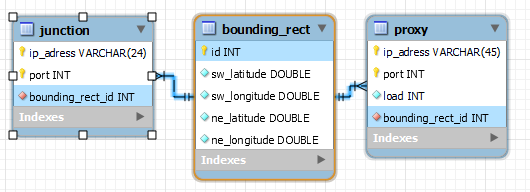
\includegraphics[width=\textwidth]{DB/DbSchema.png}
        \caption{Database Schema}
        \label{fig:Database Schema}
    \end{figure}
    \item[Parsing config files:] Specific json parser, data type converter
    \item[Creating preplanned timed actions:] Observers, Timers 
    \item[Handling user input] command line parser, signals handler
    \item[Syncronosly logging on multiple threads:] Costumizable logger
\end{description}


\pagebreak
\section{IPC}
\indent \indent
To establish the communication amoung all the executables an costum made IPC system
was develop, while using Boost Asio for socket handling. The loggic 
itself runs on 4 threads: one for keeping the context running, one for reading,
one for writing and one for notifying progress.


\begin{lstlisting}[language = C++][H]
    template<typename T>
    class Client
    {
    private:
        common::ThreadSafePriorityQueue<OwnedMessage<T>> incomingMessages_;

    protected:
        boost::asio::io_context context_;
        std::thread threadContext_;
        std::mutex mutexUpdate_;
        std::condition_variable condVarUpdate_;
        std::unique_ptr<Connection<T>> connection_;
        std::atomic<bool> shuttingDown_ = false;
        boost::asio::io_context::work idleWork_;
        LOGGER("CLIENT");
    public:
        bool connect(const utile::IP_ADRESS& host, const ipc::utile::PORT port);
        void disconnect();
        bool isConnected();
        void send(const Message<T>& msg);
        bool waitForAnswear(uint32_t timeout = 0);
        std::optional<std::pair<OwnedMessage<T>, bool>> getLastUnreadAnswear();
    }
\end{lstlisting}

\pagebreak

\begin{lstlisting}[language = C++][H]
    template <typename T>
    class Connection : public std::enable_shared_from_this<Connection<T>>
    {
    protected:
        const Owner owner_;
        std::thread threadRead_;
        std::thread threadWrite_;
        std::mutex mutexRead_;
        std::mutex mutexWrite_;
        std::condition_variable condVarRead_;
        std::condition_variable condVarWrite_;
        std::condition_variable& condVarUpdate_;
        boost::asio::io_context& context_;
        boost::asio::ip::tcp::socket socket_;
        common::ThreadSafePriorityQueue<OwnedMessage<T>>& incomingMessages_;
        common::ThreadSafePriorityQueue<Message<T>> outgoingMessages_;
        Message<T> incomingTemporaryMessage_;
        std::atomic_bool isReading_;
        std::atomic_bool isWriting_;
        std::atomic_bool shuttingDown_ = false;
        uint32_t id_;
        std::string ipAdress_;
        LOGGER("CONNECTION-UNDEFINED");

    private:
        bool readData(std::vector<uint8_t>& vBuffer, size_t toRead);
        void readMessages();
        void writeMessages();
    public:
        Owner getOwner() const;
        bool connectToServer(
            const boost::asio::ip::tcp::resolver::results_type& endpoints);
        bool connectToClient(uint32_t id);
        void disconnect();
        bool isConnected() const;
        void send(const Message<T>& msg);
    }
\end{lstlisting}

\pagebreak

\begin{lstlisting}[language = C++][H]
    template<typename T>
    class Server
    {
    protected:
        common::ThreadSafePriorityQueue<OwnedMessage<T>> incomingMessagesQueue_;
        boost::asio::io_context context_;
        std::thread threadContext_;
        std::thread threadUpdate_;
        std::condition_variable condVarUpdate_;
        std::mutex mutexUpdate_;
        std::mutex mutexMessage_;
        boost::asio::ip::tcp::acceptor connectionAccepter_;
        common::ThreadSafeQueue<uint32_t> availableIds_;
        std::map<uint32_t, std::shared_ptr<Connection<T>>> connections_;
        std::atomic<bool> shuttingDown_ = false;
        LOGGER("SERVER");
    private:
        void update();
    public:
        bool start();
        void stop();
        void waitForClientConnection(); //ASYNC
        void messageClient(std::shared_ptr<Connection<T>> client,
            const Message<T>& msg);
    protected:
        virtual bool onClientConnect(std::shared_ptr<Connection<T>> client);
        virtual void onClientDisconnect(std::shared_ptr<Connection<T>> client);
        virtual void onMessage(std::shared_ptr<Connection<T>> client,
            Message<T>& msg);
    }
\end{lstlisting}

\pagebreak

\begin{lstlisting}[language = C++][H]
    template <typename T>
    struct MessageHeader
    {
        T type{};
        uint16_t id{};
        bool hasPriority = false;
        size_t size = 0;
    };
    
    template <typename T>
    struct Message
    {
        MessageHeader<T> header{};
        std::vector<uint8_t> body;

        size_t size() const;
        void clear();
        Message<T> clone();

        friend std::ostream& operator << (std::ostream& os, 
            const Message<T>& msg);
        template<typename DataType>
        friend Message<T>& operator << (Message<T>& msg, const DataType& data)
        template<typename DataType>
        friend Message<T>& operator >> (Message<T>& msg, DataType& data)
    }
\end{lstlisting}  

%de descris tot codul
\pagebreak

\section{CarDetector}
\indent \indent
To be able to connect to the road traffic cameras and count the number of 
incoming/outgoing vehicles wrappers over OpenCV library were made. The whole process 
works as follows: it starts detecting the moving objects inside a give frame, try to 
predict their next position and once they cross a imaginary lines inside the picture
they are accounted if they were matched to be cars. To boost performance, the 
module runs on 4 threads: providing images from the camera, detecting moving objects,
classifying objects as cars and displaying the bounding boxes. The last one can be 
disable, as it is just for illustrative purposes. \\

\indent \indent
The car classification itself is 
not done by the given module due to current C++ Tensorflow - OpenCV outdated compatibility,
but by the ObjectDetectionServer written in Python. The CarDetector module just acts 
like a client and sends the actual bytes of the cropped image of the detected moving objects 
to the server. It is important to note that if, in the near future, the compatibility issues
will be fixed, it would server as a great performance upgrade to move this logic
inside the module and remove any kind of process interactions.


\section{ObjectDetectionServer} 
\indent \indent
To be able to able to detect if cars were present we made use of Tenserflow 
Object Detection API ~\ref{fig:TensorFlow}. It is a powerful framework provided by Google's TensorFlow
library that facilitates training, evaluating, and deploying object detection
models. It offers a collection of pre-trained models and tools for building custom
models to detect and localize objects in images and videos. 

% de scos poza =)
\begin{figure}[h!]
    
\includegraphics[width=\textwidth]{TensorFlow.png}
    \caption{TensorFlow (\href{https://www.vectorlogo.zone/logos/tensorflow/index.html}{Image Source} \copyright)}
    \label{fig:TensorFlow}
\end{figure}

Due to the fact that the model will be loaded by a microcontroller a
\href{https://github.com/tensorflow/models/blob/master/research/object_detection/g3doc/tf2_detection_zoo.md}{SSD MobileNet model}
was trained by using a \href{https://universe.roboflow.com/pedro-azevedo-3c9ol/bdd100k-3zgda/dataset/5}{public dataset}.
SSD MobileNet is a combination of two popular deep learning architectures:
Single Shot MultiBox Detector (SSD) and MobileNet. \\
\indent
SSD is an object detection algorithm that provides real-time object detection in images.
It achieves this by predicting the bounding boxes and class labels of multiple objects
in a single pass through a neural network. Unlike other object detection methods that
require region proposal generation, SSD directly predicts object detections at different scales
and aspect ratios.\\
\indent
MobileNet is a lightweight convolutional neural network architecture designed for efficient use on
mobile and embedded devices. It utilizes depthwise separable convolutions, which separate the spatial\
filtering and channel-wise filtering operations, reducing the computational complexity and model size.
MobileNet achieves a good balance between accuracy and efficiency, making it suitable for
resource-constrained environments.\\
\indent
By combining SSD and MobileNet, the SSD MobileNet model achieves real-time object detection on mobile
and embedded devices with limited computational resources. It provides a good trade-off between accuracy
and efficiency, making it a popular choice for various applications such as autonomous vehicles,
surveillance systems, and mobile applications requiring object detection capabilities.\\
\indent
The training was done with the use of tenserflow repository and it took about 15h
on an RTX 3060 and the model is capable of detecting cars, street lights and other
traffic related objects but it will be used just for detecting cars. The model speed
is the most important thing here beeing able to evaluate 22 frames/s, as it's
accuracy is not that great averaging 60\%. The overcome the low accuracy any object 
that is more then 50\% likely to be a car will be taken into account.\\
\indent
The model itself is loaded just once on a server, because it is a really
time consuming operation, and used whenever a new valid message is recieved.
Once the predictions are calculated, we remove the overlapping objects
detected with the help of OpenCv NMSBoxes and return just the size 
of the remaining list of objects, not the bounding boxes themself, representing 
the amount of cars detected in the given image. To keep the consistency of the IPC
implementation I imported the C++ message definitions and implemented the created
a simple implementation of a server using socket package. To further improve
the response time of the server, the request handling can be done in a asynchronous
manner, having multiple threads working on different messages for the same client. \\
\indent
Related to the actual device that will run the server, it is better to just have 
them tied down to every proxy, due to the high resource need of loading the actual 
model that can not be achived on the microcontrollers.


\pagebreak

\section{Proxy}
\indent \indent
The proxy is a wrapper over the server implementation that assures the connection
between the vechile trackers and the next junction main server they will encounter.
Every single one is connected to their own database, that contains a list of junctions,
proxys and the area covered by them. \\
\indent \indent
They way it works is preaty straight forward, if a client 
querys the proxy for the next junction it searches the database. If it finds 
a suiting junction then it sends the connection data, otherwise it redirects 
the vehicle to the closeste proxy. This process repeats itself until it 
finally reaches one valid junction or the car is out of coverage area (for 
example if the car is somewhere on a ship in the middle of the sea there is 
no reason for us to connect it to a junction).

\begin{figure}[h!]
    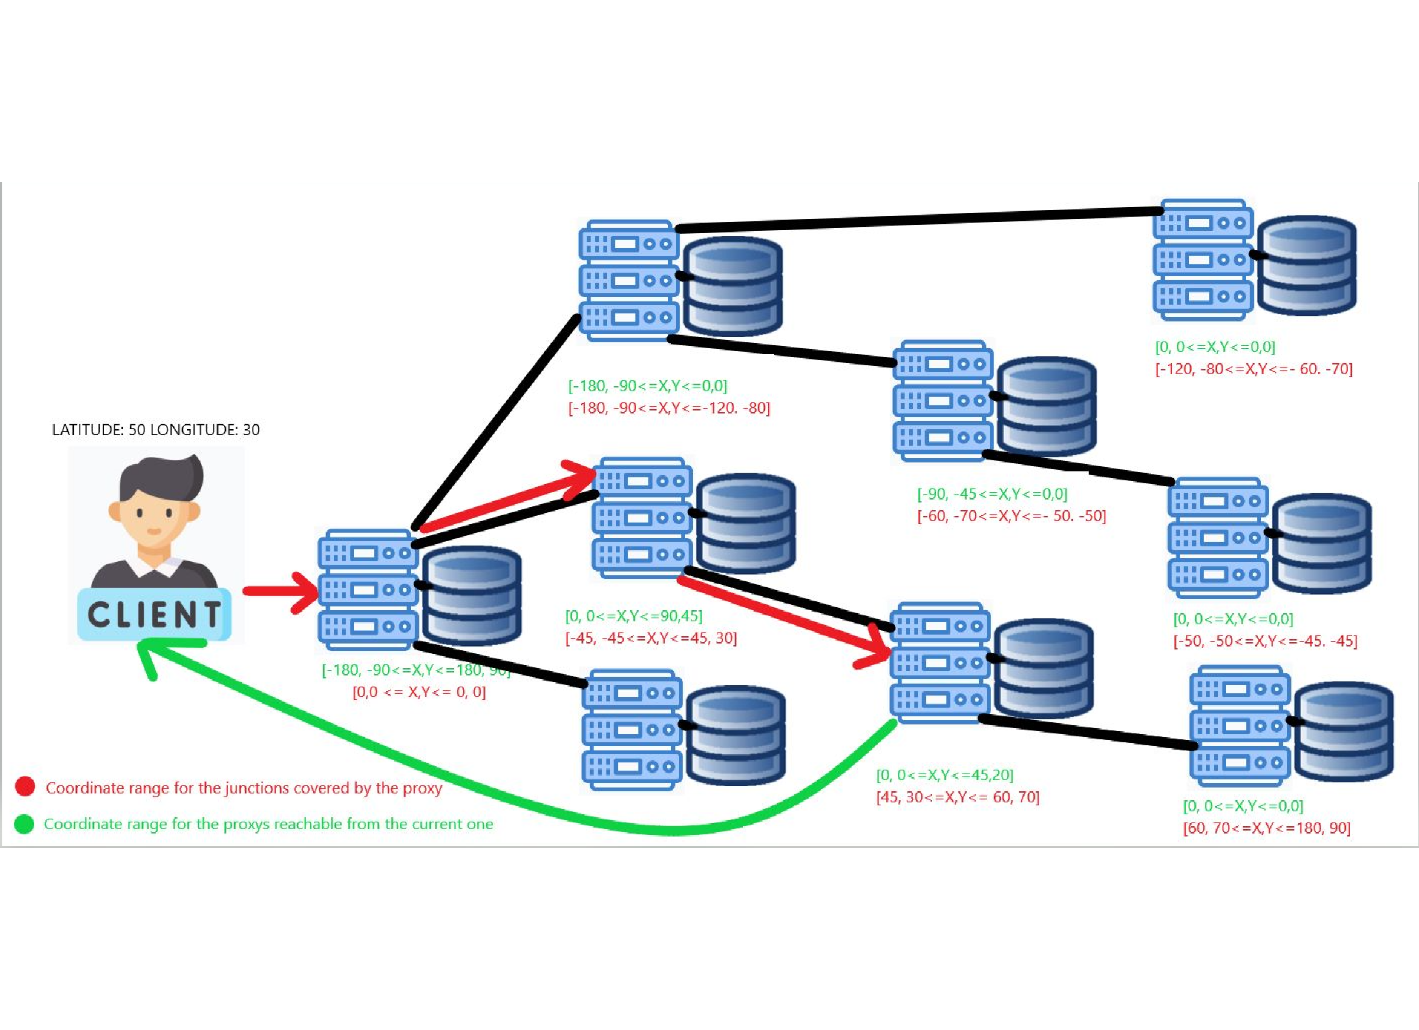
\includegraphics[width=\textwidth]{Sketches/ProxyFlowV2.png}
    \caption{Proxy querys flow}
    \label{fig:Proxy querys flow}
\end{figure}

The servers themself have a range of coordinate values for the covered junctions
and a range of coordinate values for the known connected subproxys. The coordinate 
range of the know connected proxys lessens the more you go down the connection tree 
until an enpoint is reached, marked with range {0,0} \textless = \textgreater {0,0}.
(Figure ~\ref{fig:Proxy querys flow}). If we still don't got 
an answear from the proxy containing a junction that means that we are out of reach 
and the client will just stop. Like this, the more servers we will have to spread our 
junction data, the faster the communication will be, as the client doesn't necessarily
need to interogate the main server, it can interogate any of the servers.
\pagebreak


\section{JunctionMainServer}

\indent \indent
The executable is a wrapper over the server implementation that manages the traffic states.
It keeps track of the incoming vehicles and times out each and every traffic state. The 
implementation itself is thought to be a state machine, with the states represented by the 
traffic states and the events being timer expire events. Each state has associated to it 
a timer that decreases normally or when an incoming vehicle is detected. Whenever we 
are in a given state, it's corresponding timer is frozen and afterwards reseted.

%de descris pe scurt fisierul de configurare
\begin{lstlisting}[language = C++][H]
{ 
    "server": { "ip": "127.0.0.1", "port": 5000 },
    "maxWaitingTime": 2,
    "usingLeftLane": true,
    "lanes": { 
        "top": "keyword1", "down": "keyword2",
        "left": "keyword3", "right": "keyword3"
    } 
}
\end{lstlisting}

Both the timer for the green light and the ones attached to each lane 
dinamically update based on the traffic. To describe the way this is 
done we must first analise what increasing/decreasing the waiting time 
means for our system and also what could cause this scenario. 
What we would wish to achive is that every time a state ends X
drivers have passed the junction. To do so, we control the amount of 
time a driver has to pass the junction. Also, the most important part 
is to minimize the amount of time those cars have to wait to pass the 
junction. Like so, we would want to increase/decrease the green light 
timer as well as the driver waiting timer attached to each lane. 
Figure ~\ref{fig:Timer Increase/Decrease Impact} illustrates
what negative effects playing arround with those timers would bring
to our system.

\begin{figure}[h!]
    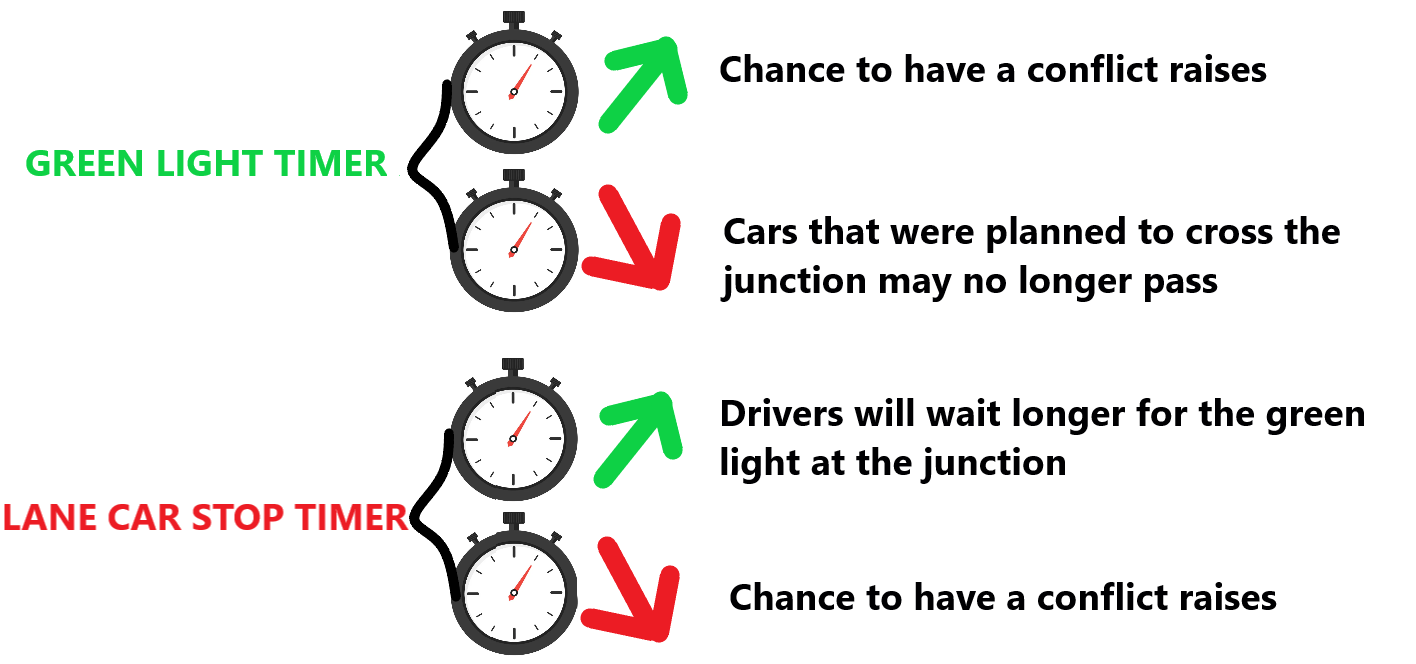
\includegraphics[width=\textwidth]{Sketches/TimerIncreaseDecreaseImpact.png}
    \caption{Timer Increase/Decrease Impact}
    \label{fig:Timer Increase/Decrease Impact}
\end{figure}

To achive the desired traffic flow described above while minimizing
the waiting time as much as we can we must be aware of 2 things:
avoiding less cars passing the junction; avoiding conflicting states

\begin{figure}[h!]
    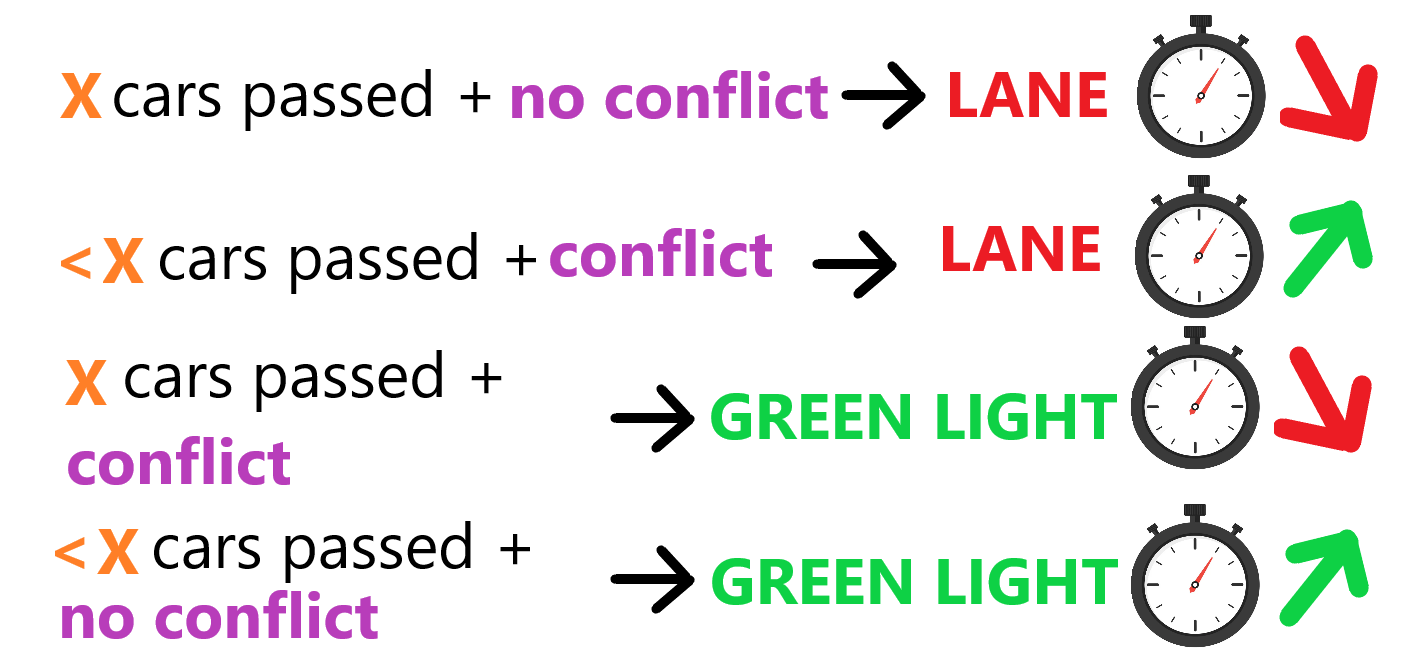
\includegraphics[width=\textwidth]{Sketches/FaultyScenariosHandling.png}
    \caption{Faulty Scenarios Handling}
    \label{fig:Faulty Scenarios Handling}
\end{figure}

\indent
Figure ~\ref{fig:Faulty Scenarios Handling} illustrates how 
we actually handle each combination of those scenarios. The way we determine if enough vehicles passed is by 
tracking the actual cars. Due to high complexity of image 
comparison, this number is based only on the VehicleTrackers 
input, so TrafficObserver client does not contribute to this process 
and significant decreases in waiting time can be seen only for the 
cars that are capable of using the VehicleTracker client.\\
\indent
As for the way the lane timer decreases when a new vehicle is
detected we will have a value that constanly increases the more cars 
are waiting. We also keep in mind an average of cars 
waiting to pass the junction and whenever the value is surpassed 
we start to drastically increase the amount of time decreased 
for the corresponding timer.\\
\indent
During the testing of the given module it was observed that traffic tends to keep it's 
normal flow, there is no jumping between traffic states unless a large inflow of cars is 
detected. Even if this happens, after the required jump transitions, traffic states will 
be normalized back to their initial flow definition.

\pagebreak
\section{TrafficObserver}
\indent \indent
The executable is a wrapper over the client implementation that combines
cardetection functionalities. On startup it recieves a keyword for the junction to be able
to determine what lane provided the incoming car message. To be able to run 
the executable itself you will need to provide a camera as well as a way to 
connect to the network, for example a zigbee. For testing porposes a
video was provided instead of linking directly to a camera. ~\ref{fig:Running client samples}

% de adaugat nume si descris eventual
\begin{figure}[h!]
    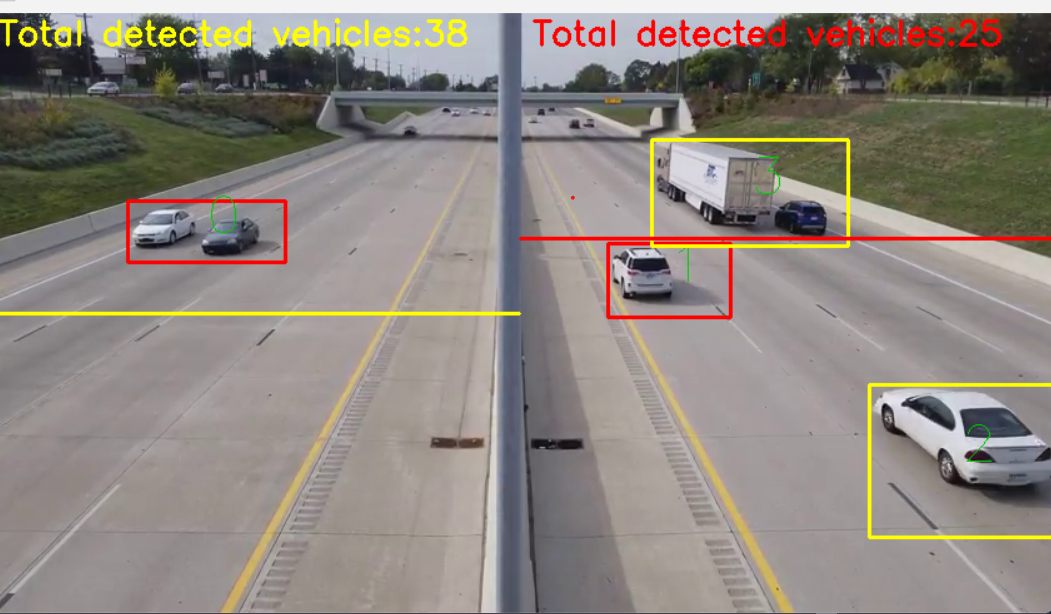
\includegraphics[width=\textwidth]{TrafficDetectionRunningExample.png}
    \label{fig:Running client sample}
\end{figure}

\begin{figure}[h!]
    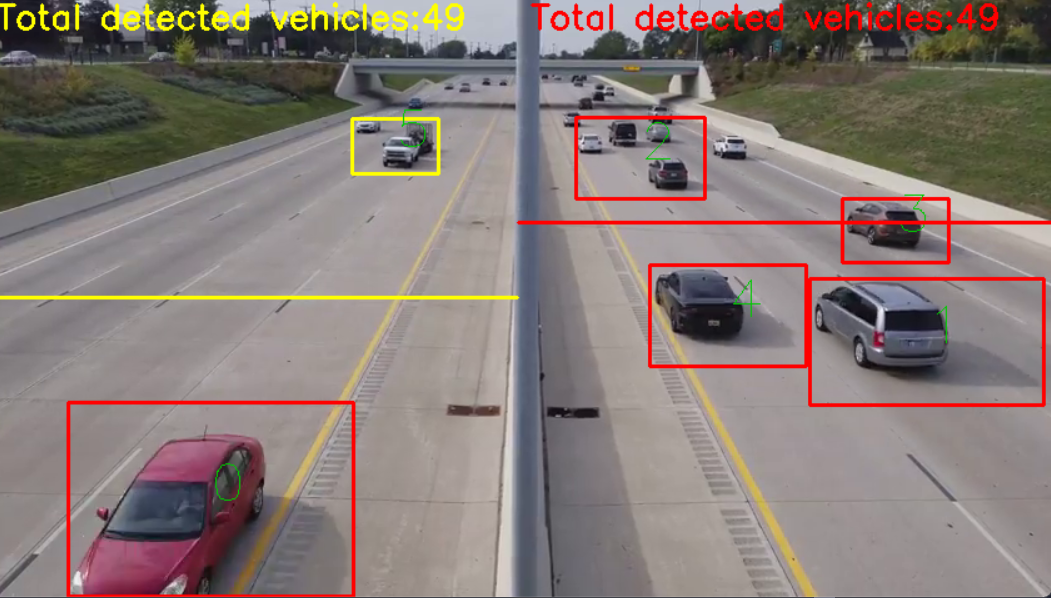
\includegraphics[width=\textwidth]{TrafficDetectionRunningExample2.png}

    \label{fig:Running client samples}
\end{figure}

\pagebreak
\section{VehicleTracker}
\indent \indent
The executable is a wrapper over the client. On startup it tries loading a
config file that contains an ordered list with the previous queried proxies.
If not present, it will just interogate the main server. Once the application
shuts down a config file will be saved with all the queried proxys, so it will
almost always load a config file.

\begin{lstlisting}[language = C++][H]
{
    "proxys": [
    { "ip_adress": "127.0.0.1","port": 6000},
    { "ip_adress": "127.0.0.5","port": 5000}]
}
\end{lstlisting}

The executable aims to be downloaded on each car system by the manufacturer
and it requires a GPS module to be pressent as well as a wifi module. Messages
start to be sent only when the vehicle itself is moving. To be able to
determine this as well as it's heading GPS data is manually parsed, extracting
latitude and longitude from NMEA GPGLL, GPGGA and GPRM inputs. For testing
purposes data was already written inside a file and passed trough a pipe to the
application. The data itself was taken from a \href{https://github.com/ChrisvdHoorn/NMEA_message_GPS_data}{public repository}.

\indent \indent
We first query the last visited proxy. If we are out of reach, we move up the proxy list
until eventually we get valid junction connection data ~\ref{fig:Proxy junction data reply} or we get back to
the root of the connection tree(the main server). If we have reached the root node, 
the process of searching for a junction without a config file restarts. Once we got the 
connection data we notify the junctions whenever we aproach/disconnect from it. When we 
have passed a junction the whole process restarts from the last queried proxy.

\begin{figure}[h!]
    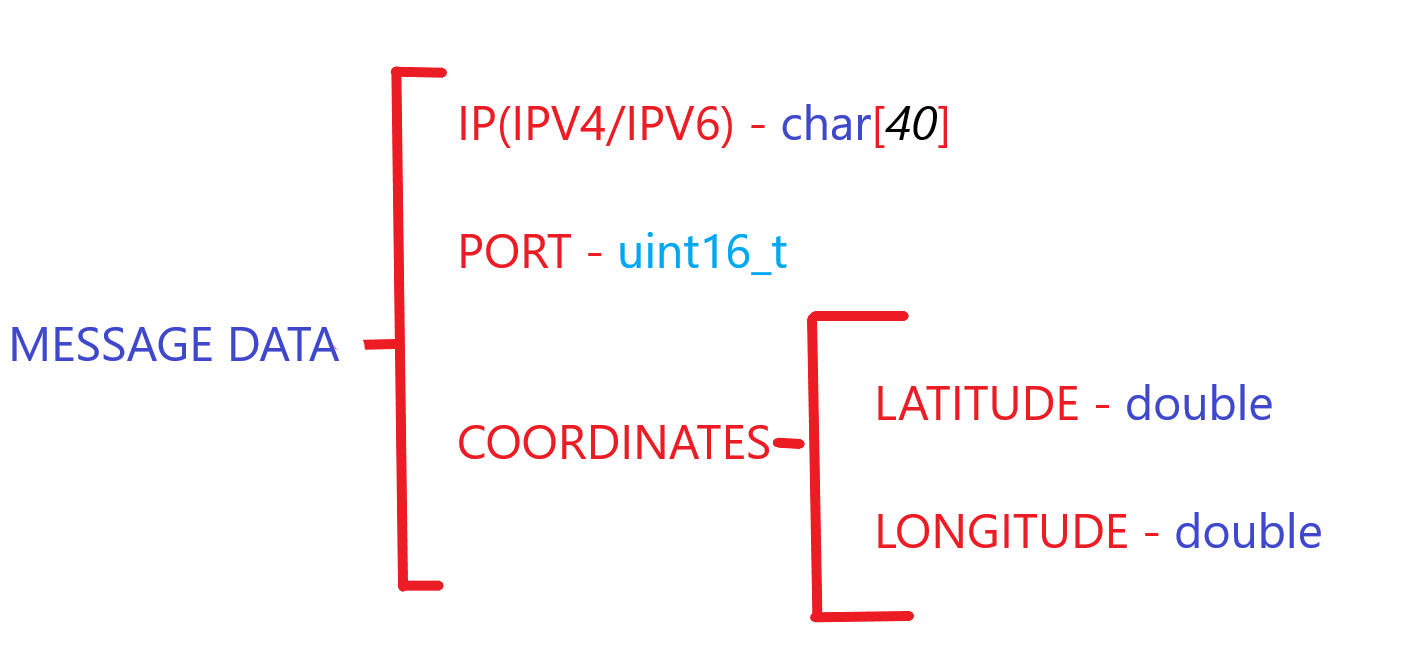
\includegraphics[width=\textwidth]{Sketches/ProxyJunctionMessage.png}
    \caption{Proxy junction data reply}
    \label{fig:Proxy junction data reply}
\end{figure}

%de impartit in mai multe subcapitole "Conclusions and Further Directions"
\chapter{Conclusions and Further Directions}
\indent \indent
In this paper, through an analysis of existing research,
implementation examples, and emerging trends, we have gained valuable
insights into the effectiveness and potential of traffic management
systems. With the data collected, we have provided a new alternative 
way of managing traffic by defining and implementing a new traffic 
system that we believe will significantly improve traffic flow. \\
\indent
The new system itself attempts to bennefit on already existing V2V and V2I
communication and provides an IPC based system with multiple clients, servers
and proxys that can achive data car collection and processing on a global scale.
It servers as a new economic aproach, due to the low hardware requirements,
and acts as a bridge between current traffic flow handling and a fully 
DSRC signal based traffic control system that we believe will be the 
future of traffic handling systems. \\
\indent 
We mainly focused on the performance part to be able to provide
the smoothest traffic conditions that we could offer at minimal costs,
so many other branches, especially the vulnerability defense area,
were mostly neglected. \\
\indent
One thing that should be done in the near future, if the system will be chosen to be 
applied in real time scenarios would be to implement a securtiy 
layer or protocol that would prevent attackers from distur
bing the 
normal traffic flow. Also, right now messages are not encrypted and 
can be captured by anyone, so another step into protecting our system 
would be to add a public-private key mechanism or try adding some 
security protocols like Cerberus. \\
\indent 
Another thing that should be done before deploying our system on a 
global level is to create a real time test environment, as for now,
no real-time testing was done, so the system may or may not fail. 
We tried to provide as close to reality data to our system, but there 
are almost always room for error when dealing with such vast subjects
like traffic management

\pagebreak
\printbibliography

\end{document}